% A LaTeX template for MSc Thesis submissions to 
% Politecnico di Milano (PoliMi) - School of Industrial and Information Engineering
%
% S. Bonetti, A. Gruttadauria, G. Mescolini, A. Zingaro
% e-mail: template-tesi-ingind@polimi.it
%
% Last Revision: October 2021
%
% Copyright 2021 Politecnico di Milano, Italy. NC-BY

\documentclass{Configuration_Files/PoliMi3i_thesis}

%------------------------------------------------------------------------------
%	REQUIRED PACKAGES AND  CONFIGURATIONS
%------------------------------------------------------------------------------

% CONFIGURATIONS
\usepackage{parskip} % For paragraph layout
\usepackage{setspace} % For using single or double spacing
\usepackage{emptypage} % To insert empty pages
\usepackage{multicol} % To write in multiple columns (executive summary)
\setlength\columnsep{15pt} % Column separation in executive summary
\setlength\parindent{0pt} % Indentation
\raggedbottom  

% PACKAGES FOR TITLES
\usepackage{titlesec}
% \titlespacing{\section}{left spacing}{before spacing}{after spacing}
\titlespacing{\section}{0pt}{3.3ex}{2ex}
\titlespacing{\subsection}{0pt}{3.3ex}{1.65ex}
\titlespacing{\subsubsection}{0pt}{3.3ex}{1ex}
\usepackage{color}
\usepackage[outdir=./]{epstopdf}

% PACKAGES FOR LANGUAGE AND FONT
\usepackage[english]{babel} % The document is in English  
\usepackage[utf8]{inputenc} % UTF8 encoding
\usepackage[T1]{fontenc} % Font encoding
\usepackage[11pt]{moresize} % Big fonts

% PACKAGES FOR IMAGES
\usepackage{graphicx}
\usepackage{transparent} % Enables transparent images
\usepackage{eso-pic} % For the background picture on the title page
%\usepackage{subfigure}
%\usepackage{subfig} % Numbered and caption subfigures using \subfloat.
\usepackage{tikz} % A package for high-quality hand-made figures.
\usetikzlibrary{}
\usetikzlibrary{positioning}
\graphicspath{{./Images/}} % Directory of the images
\usepackage{caption} % Coloured captions
\usepackage{subcaption}
\usepackage{xcolor} % Coloured captions
\usepackage{amsthm,thmtools,xcolor} % Coloured "Theorem"
\usepackage{float}
\usepackage{wrapfig}

% STANDARD MATH PACKAGES
\usepackage{amsmath}
\usepackage{amsthm}
\usepackage{amssymb}
\usepackage{amsfonts}
\usepackage{bm}
% \usepackage{enumerate}
\usepackage[inline]{enumitem}
\usepackage[overload]{empheq} % For braced-style systems of equations.
\usepackage{fix-cm} % To override original LaTeX restrictions on sizes

% PACKAGES FOR TABLES
\usepackage{tabularx}
\usepackage{longtable} % Tables that can span several pages
\usepackage{colortbl}

% PACKAGES FOR ALGORITHMS (PSEUDO-CODE)
\usepackage{algorithm}
\usepackage{algpseudocode}
%\usepackage{algorithmic}

% For inserting code
\usepackage{listings}
\usepackage{xcolor}
\usepackage{minted}
\usemintedstyle{pastie}


% PACKAGES FOR REFERENCES & BIBLIOGRAPHY
\usepackage[colorlinks=true,linkcolor=black,anchorcolor=black,citecolor=black,filecolor=black,menucolor=black,runcolor=black,urlcolor=black]{hyperref} % Adds clickable links at references
\usepackage{cleveref}
\usepackage[square, numbers, sort&compress]{natbib} % Square brackets, citing references with numbers, citations sorted by appearance in the text and compressed
\bibliographystyle{abbrvnat} % You may use a different style adapted to your field

% OTHER PACKAGES
\usepackage{pdfpages} % To include a pdf file
\usepackage{afterpage}
\usepackage{lipsum} % DUMMY PACKAGE
\usepackage{fancyhdr} % For the headers
\usepackage{comment} % Comment part of code
\fancyhf{}

% For displaying SVG files
\usepackage{svg}

% Input of configuration file. Do not change config.tex file unless you really know what you are doing. 
\input{Configuration_Files/config}

%----------------------------------------------------------------------------
%	NEW COMMANDS DEFINED
%----------------------------------------------------------------------------

% EXAMPLES OF NEW COMMANDS
\newcommand{\bea}{\begin{eqnarray}} % Shortcut for equation arrays
\newcommand{\eea}{\end{eqnarray}}
\newcommand{\e}[1]{\times 10^{#1}}  % Powers of 10 notation

\newcommand{\fil}[1]{{\textcolor{blue}{[\textbf{Filippo}: #1]}}}
\newcommand{\dan}[1]{{\textcolor{green}{[\textbf{Danilo}: #1]}}}

%----------------------------------------------------------------------------
%	ADD YOUR PACKAGES (be careful of package interaction)
%----------------------------------------------------------------------------

%----------------------------------------------------------------------------
%	ADD YOUR DEFINITIONS AND COMMANDS (be careful of existing commands)
%----------------------------------------------------------------------------

%----------------------------------------------------------------------------
%	BEGIN OF YOUR DOCUMENT
%----------------------------------------------------------------------------

\begin{document}



\fancypagestyle{plain}{%
\fancyhf{} % Clear all header and footer fields
\fancyhead[RO,RE]{\thepage} %RO=right odd, RE=right even
\renewcommand{\headrulewidth}{0pt}
\renewcommand{\footrulewidth}{0pt}}

%----------------------------------------------------------------------------
%	TITLE PAGE
%----------------------------------------------------------------------------
\hypersetup{pageanchor=false}
\pagestyle{empty} % No page numbers
\frontmatter % Use roman page numbering style (i, ii, iii, iv...) for the preamble pages

\puttitle{
	title=Anomaly Detection via learned models and preference trick, % Title of the thesis
	name=Danilo Catone, % Author Name and Surname
	course=Computer Science Engineering \newline
	Ingegneria Informatica, % Study Programme (in Italian)
	ID  = 951402,  % Student ID number (numero di matricola)
	advisor= Prof. Luca Magri, % Supervisor name
	coadvisor={Giacomo Boracchi, Filippo Leveni}, % Co-Supervisor name, remove this line if there is none
	academicyear={2021-22},  % Academic Year
} % These info will be put into your Title page 

%----------------------------------------------------------------------------
%	PREAMBLE PAGES: ABSTRACT (inglese e italiano), EXECUTIVE SUMMARY
%----------------------------------------------------------------------------
\startpreamble
\setcounter{page}{1} % Set page counter to 1

% ABSTRACT IN ENGLISH
\chapter*{Abstract} 
\label{ch:abstract_en}

\hspace{5pt}
Anomaly Detection is a field of data mining applied in numerous contexts such as quality inspection, fraud detection, and medicine, that seeks to detect anomalies in a dataset, defined as those instances that do not have a well-defined behavior or that deviate from usual behavior.

\hspace{5pt}
In this thesis we focus on anomalies in datasets containing structured normal points, i.e., those in which normal points follow well-defined pattern, while points not following the pattern are considered anomalous. 
\begin{comment}
    \newline
    As an example, consider a dataset containing information about the position of the joints of a mechanical robot; the joints are constrained in the movements and can occupy only certain regions of the space, following predetermined patterns of movements. In this context, correct positions will follow the pattern and will be considered normal points in the space; anomalous positions, instead, indicate a wrong position of a joint not following the pattern, which could cause breakdowns. \newline
    Therefore, it is very important being able to detect this anomalies in order to mitigate the possibility of unexpected events.
\end{comment}

\hspace{5pt}
In this context we want to extend PIF, a model-based anomaly detection algorithm that embeds the points in the dataset in the preference space and applies iVor algorithm on it, in order to compute an anomaly score for each instance. The embedding in the preference space is done through a pool of models sampled from data, containing patterns of which we assume to know the formulation.

\hspace{5pt}
We will show that is possible to build an ensemble of more general models that extract patterns autonomously, directly from data, without the knowledge of the patterns to search for. Therefore, we will demonstrate 
\begin{enumerate*}[label=(\roman*)]
    \item that is possible to locally approximate normal data with a model, and
    \item that the models can learn the patterns without any information on the type of pattern.
\end{enumerate*}
This is possible thanks to two types of Neural Networks, auto-encoders and self-organizing maps, that learn the pattern to search instead of fixing it as in PIF.

\hspace{5pt}
We tested our algorithm on publicly available synthetic datasets, comparing it with two state-of-the-art density-based methods such as iFor and LOF, showing that our algorithm is superior in terms of ROC AUC on all datasets; we also explored different models and architectures for each model, looking for the right hyper-parameters.

\paragraph{}
\textbf{Keywords}: anomaly detection, neural networks, preference embedding, self organizing maps, auto encoders

% ABSTRACT IN ITALIAN
\chapter*{Abstract in lingua italiana}
L'Anomaly Detection è un campo del data mining applicato in numerosi contesti, come l'ispezione della qualità, il rilevamento delle frodi e in medicina, che cerca di individuare le anomalie presenti in un set di dati, definite come quelle istanze che non hanno un comportamento ben definito o che si discostano dal comportamento abituale.

\hspace{5pt}
In questa tesi ci concentriamo sulle anomalie nei set di dati contenenti punti normali strutturati, cioè quelli in cui i punti normali seguono schemi (pattern) ben definiti, mentre i punti che non seguono gli schemi sono considerati anomali.

\hspace{5pt}
In questo contesto, vogliamo estendere PIF, un algoritmo di Anomaly Detection che incorpora i punti del set di dati nello spazio delle preferenze e applica Voronoi Isolation Forest su di essi, al fine di calcolare un punteggio di anomalia per ogni istanza. L'incorporazione nello spazio delle preferenze avviene attraverso un insieme di modelli campionati dai dati, contenenti pattern di cui si presume di conoscere la formulazione.

\hspace{5pt}
Dimostreremo che è possibile costruire un ensemble di modelli più generali che estraggono i pattern autonomamente, direttamente dai dati, senza la conoscenza dei pattern da ricercare. Pertanto, dimostreremo
\begin{enumerate*}[label=(\roman*)]
    \item che è possibile approssimare localmente i dati normali con un modello, e
    \item che i modelli possono apprendere i pattern senza alcuna informazioni sul tipo di modello.
\end{enumerate*}
Questo è possibile grazie a due tipi di reti neurali, gli auto-encoders e le self-organizing maps, che apprendono il modello da ricercare invece di fissarlo come nel PIF.

\hspace{5pt}
Abbiamo testato il nostro algoritmo su dataset sintetici disponibili pubblicamente, confrontandolo con due metodi dello stato dell'arte basati sulla densità come iFor e LOF, dimostrando che il nostro algoritmo è superiore in termini di ROC AUC su tutti i dataset; abbiamo inoltre esplorato diversi modelli e architetture per ogni modello, alla ricerca degli hyper-parametri giusti.

\paragraph{}
\textbf{Parole chiave}: rilevamento di anomalie, reti neurali, preference embedding, self-organizing maps, auto-encoder


% ACKNOWLEDGEMENTS
\chapter*{Acknowledgements}
\paragraph{}
Prima di procedere con la trattazione, vorrei dedicare qualche riga a tutti coloro che mi sono stati vicini in questo percorso di crescita personale e professionale.

\paragraph{}
In primis, un ringraziamento al mio relatore Luca, che in questi sette mesi di lavoro ha saputo guidarmi, con suggerimenti pratici, nelle ricerche e nella stesura dell’elaborato.
Grazie anche al mio correlatore Filippo per i suoi preziosi consigli, per le ore passate a rimurginare sui concetti in cerca del lampo di genio e per avermi suggerito puntualmente le giuste modifiche da apportare alla mia tesi.

\paragraph{}
Ringrazio di cuore i miei genitori e mio fratello, senza i quali non sarei quello che sono oggi. Mi avete insegnato cosa significa fare sacrifici e lavorare per ottenere ciò che si desidera, cosa significa non mollare e tenere duro anche nei momenti difficili. Mi siete sempre stati accanto, mi avete supportato e sopportato. Non mi avete mai fatto sentire smarrito, con voi affianco sapevo bene dove andare.

\paragraph{}
Ringrazio la mia fidanzata, Giulia, per avermi regalato i momenti e le emozioni più belli. Grazie per il tuo sostegno, senza il quale non sarei arrivato a questo momento; grazie per avermi dato la forza di andare avanti quando questa non c'era più. Semplicemente, grazie di essere qui con me; quando siamo insieme, sò che tutto è al suo posto.

\paragraph{}
Ringrazio tutti gli zii, tutti i cugini e la nonna, sarete sempre un punto di riferimento per me. Mi avete visto crescere e mi avete accompagnato in questo viaggio, viziandomi quando necessario. Anche se ormai non trascorriamo più tanto tempo insieme, sarete sempre una parte di me e sono orgoglioso di avere una famiglia come voi.

\paragraph{}
Come non ringraziare poi gli amici di una vita, con i quali ho trascorso giornate indimenticabili. Grazie per esserci sempre stati, per essere sempre pronti a tirarmi su quando tutto va male. Grazie a voi sò cosa significa essere un vero amico e cosa significa avere una seconda famiglia. Anche se ultimamente ognuno sta prendendo la propria strada, rimarremo sempre uniti.

\paragraph{}
Per ultimo, ma non per importanza, vorrei ringraziare me stesso. Voglio ringraziarmi per aver sempre creduto in me, voglio ringraziarmi per tutto questo duro lavoro, voglio ringraziarmi per non essermi mai fermato e non aver mai saziato la mia fame. Ringrazio me stesso per il semplice fatto di essere me.
% LIST OF SYMBOLS
% Write out the List of Symbols in this page
\chapter*{List of Symbols} % You have to include a chapter for your list of symbols (
\begin{table}[H]
    \centering
    \begin{tabular}{ll}
        \textbf{Variable} & \textbf{Description} \\\hline\\[-9px]
        $\mathcal{D}$ & generic dataset \\[2px]
        $\mathcal{M}$ & generic manifold \\[2px]
        $\mathcal{N}$ & set of normal points \\[2px]
        $\mathcal{A}$ & set of anomalies \\[2px]
        $\textbf{p}$ & a generic point of the dataset \\[2px]
        $\mathcal{MSS}$ & the Minimum Sample Set \\[2px]
        $\rho$ & size of Minimum Sample Set \\[2px]
        $\tau$ & inlier threshold \\[2px]
        AE & generic auto-encoder \\[2px]
        SOM & generic self organizing map \\[2px]
        
    \end{tabular}
\end{table}
\hypersetup{pageanchor=true}
%----------------------------------------------------------------------------
%	LIST OF CONTENTS/FIGURES/TABLES/SYMBOLS
%----------------------------------------------------------------------------

% TABLE OF CONTENTS
\thispagestyle{empty}
\tableofcontents % Table of contents 
\thispagestyle{empty}
\cleardoublepage

%-------------------------------------------------------------------------
%	THESIS MAIN TEXT
%-------------------------------------------------------------------------
% In the main text of your thesis you can write the chapters in two different ways:
%
%(1) As presented in this template you can write:
%    \chapter{Title of the chapter}
%    *body of the chapter*
%
%(2) You can write your chapter in a separated .tex file and then include it in the main file with the following command:
%    \chapter{Title of the chapter}
%    \input{chapter_file.tex}
%
% Especially for long thesis, we recommend you the second option.

\addtocontents{toc}{\vspace{2em}} % Add a gap in the Contents, for aesthetics
\mainmatter % Begin numeric (1,2,3...) page numbering


\chapter{Introduction}
\label{ch:introduction}
\paragraph{}
From financial fraud detection to healthcare insurance, anomaly detection is one of the most studied problem in data analysis and inspired the research towards the design of statistical or machine learning algorithms. \newline
The objective of this task is to identify \textbf{anomalies}, defined as a dataset instance that deviates from expected behavior, or is otherwise distinct from other instances. \newline
In the literature, \textit{normal} points are data instances that lie in denser regions or that follow a certain structure, while \textit{anomalies} fall in low-density regions or that do not follow any structure.

\paragraph{}
Applications for anomaly detection algorithms are fraud detection, cyber-security intrusions, insurance forgery and other fraudulent or hazardous activities, but they are also employed in other contexts such as finding anomalous pixels inside an image or, in quality inspection, understand if a component is faulty or not. \newline
The methods to solve this problems has been used in a range of industries in order to advance IT safety and detect potential abuse or assaults, since anomalies in information systems frequently indicate some security breaches or violations. Thus, anomaly detection methods can also guarantee a greater level of security. 

\begin{figure}[tb]
  \begin{center}
    \includesvg[width=0.6\textwidth]{Images/sinusoidal.svg}
  \end{center}
  \caption{Example of structured dataset $\mathcal{D} \in \mathbb{R}^2$. \textbf{Normal} points are shown in \textbf{orange}, while \textbf{anomalies} are shown in \textbf{blue}. The pattern in the dataset is a sinusoidal function $f(x) = y = sin(x)cos(x)$. Anomalies are random points that do not follow any pattern, laying in the same space of the normal points.}
\label{fig:sinusoidal}
\end{figure}

\paragraph{}
In this thesis we will mainly focus on structured datasets, in which anomalies are generated from a different structure, or pattern, with respect to the one that generated normal points. In this case, the density of the points can be unimportant to identify anomalies because it does not say anything about the pattern. There are situations in which the instances of the dataset with a normal behaviour follow a precise pattern, e.g. can be plotted on a line or on a circle or on more complex figures, while anomalies are outside this structures. In other words, the normal behavior is guided by an unknown pattern, or manifold, and anomalies lie outside this manifold and do not conform to any specific behavior. As an example, in figure \ref{fig:sinusoidal} is shown a dataset with a sinusoidal pattern: orange points follow the pattern, being normal; the blue ones, instead, do not have a structure and represents the anomalies.


In this context, Anomaly Detection can be seen as a pattern-recognition problem, solved using parametric techniques, in which we need to identify the patterns that generated the data in order to understand if a point follows one of them or it is an anomaly not following any pattern. \newline
The challenging element is that the manifolds are unknown, and we need to identify the anomalies in the dataset in order to understand the structures. But we need the original pattern in order to identify the anomalies.
In this context, we have developed a \textbf{novel} algorithm able at identifying the patterns in the data using \textbf{robust model regression} and the \textbf{preference embedding}. 

\begin{comment}
    \paragraph{}
    Consequently, the formation of patterns is a necessary first step in the detection process, followed by the identification of the units that violate those patterns.
    Each method specifies a distance function, such as the Euclidean distance for numerical data, that can be used to calculate how far away and so unique an instance is from other instances. \newline
    As a result, according to the description given above, one may define an "anomalous" point as one that deviates from the norm, or the expected normal behavior or value usual for a given dataset. The data unit could be out of proportion to the majority of the data, which would cause it to deviate from the average values. When the dataset is visualized, an anomalous data unit will stand out significantly from the other data units, which are all closely spaced. \newline
    
    \paragraph{}
    However, in reality, anomaly identification is still difficult because most anomalies have unclear definitions. The term "global anomaly" typically refers to a unit that is significantly different from the dataset from any perspective. Both automatically and manually, it is simple to recognize. Local anomalies, however, or little clusters of aberrant data that are relatively close to the main dataset or values that differ from it insignificantly, are the problem. These ambiguities suggest that rather than using one of the two labels—normal or anomalous—a more sensitive method of finding anomalies is through their scoring in terms of anomaly intensity.
\end{comment}

\section{Use cases}
\paragraph{}
In order to give a context to this task, we show here some use cases in which Anomaly Detection is the key to avoid bad consequences.

\begin{itemize}
    \item \textbf{Cyber-intrusion}: Cyber-security is usually guaranteed with the help of network
        behavior anomaly detection (NBAD) technology \cite{ae_examples_nbda}. The system analyzes packet signatures to detect security threats and block incoming/outgoing data that is compromised. NBAD also conducts continuous network monitoring to detect suspicious events or trends
    \item \textbf{Fraud}: Graph-based anomaly detection (GBAD) is used to prevent fraud with
        credit cards, bank accounts, and insurance \cite{ae_examples_fraud}. Machine Learning systems also enable online banking fraud with the help of behavioral biometrics that also detects anomalies in consumer spending in real-time \cite{ae_examples_behaviour}.
    \item \textbf{Medical anomaly detection}: Outlier identification has been applied in clinical
        settings in a variety of ways. For instance, the density-based clustering method can be applied to patient careflow log analysis \cite{ae_examples_patient_careflow} to see whether the particular patient's careflow trace is anomalous. Anomaly detection in medical image analysis is helpful in accurate diagnostics, while treatment plan analysis may help determine potentially fatal errors in the treatment plans \cite{ae_examples_treatment}.
    \item \textbf{Industrial damage}: In the conditions of industrial automation, anomaly
        detection systems use data coming from numerous sensors to identify any malfunctions in the machinery \cite{ae_examples_machine_failure} \cite{ae_examples_acoustic_failure}, thus able to detect abnormalities early to prevent further damage or manufacturing defects.
    \item \textbf{Image processing}: The ability of anomaly detection systems to compare and
        analyze images allows accurate fraud detection in banking and insurance (when one recipient of a service submits duplicate reimbursement claims or when fraudsters try to receive reimbursement on fake claims)
    \item \textbf{Stock trading}: Anomaly detection algorithms deal quite well with the big masses
        of unstructured data in the stock exchanges, be it regular stocks or cryptocurrencies. ML systems classify the available data about price movements and sales volumes to detect anomalies and give alerts to the users about price outliers. This information may be instrumental in trading decision-making.
\end{itemize}

\section{Thesis Structure}
The rest of the thesis will be organized as follows: in Chapter \ref{ch:background} we present some background concepts that can help the reader to understand the basic concepts used in our solution. In Chapter \ref{ch:state_of_art} we show a brief taxonomy of Anomaly Detection algorithms, explaining the idea behind the families of algorithms and explaining in-depth the algorithms used in our comparisons. \newline
In Chapter \ref{ch:proposed_solution} we explain our solution to the problem, giving a formal definition of it and describing how and why we developed this method. In Chapter \ref{ch:experiments} we will show the results obtained by our algorithm, comparing it to the State-of-Art algorithms on synthetic datasets.
Finally, in Chapter \ref{ch:conclusions} we make our final thought about the project and explain how it can be improved and which are the next steps.
\newpage
% \chapter{Experiments (Temporary)}
Here I will present some content that will be used in other chapters. In particular, I will present the datasets used, some plots of best AUC Rocs and some tables summarizing the results obtained until now.

\section{2D}

\begin{table}[h]
    \centering
    \def\arraystretch{1.5}
    \begin{tabular}{|| c | c | c | c | c ||}
    \hline
         & |X| & |A| & |S| & |$S_1$|, ..., |$S_k$|  \\
    \hline \hline
    stair3 & 800 & 400 & 400 & $|S_1| = 272$, $|S_i| = 64$ $\forall i \in \{2, 3\}$ \\
    \hline
    stair4 & 400 & 200 & 200 & $|S_i| = 50$ $\forall i \in \{1, ..., 4\}$ \\
    \hline
    star5 & 500 & 250 & 250 & $|S_i| = 50$ $\forall i \in \{1, ..., 5\}$ \\
    \hline
    star11 & 1100 & 550 & 550 & $|S_i| = 50$ $\forall i \in \{1, ..., 11\}$ \\
    \hline
    circle3 & 1000 & 500 & 500 & $|S_1| = 376$, $|S_i| = 62$ $\forall i \in \{2, 3\}$ \\
    \hline
    circle4 & 400 & 200 & 200 & $|S_i| = 50$ $\forall i \in \{1, ..., 4\}$ \\
    \hline
    circle5 & 500 & 250 & 250 & $|S_i| = 50$ $\forall i \in \{1, ..., 5\}$ \\
    \hline
    lines & 800 & 400 & 400 & $|S_i| = 100$ $\forall i \in \{1, ..., 4\}$ \\
    \hline
    parables & 600 & 300 & 300 & $|S_i| = 100$ $\forall i \in \{1, ..., 3\}$ \\
    \hline
    \end{tabular}
    \caption{Synthetic (2D) datasets settings}
    \label{tab:syn_2d_ds_settings}
\end{table}

\begin{table}[h]
    \centering
    \def\arraystretch{1.5}
    \begin{tabular}{|| c | c | c | c | c | c | c ||}
    \hline
         & 0.1 & 0.5 & 1 & 1.5 & 2 & 2.5  \\
    \hline \hline
    AutoEncoder & 0.99 & 0.99 & 0.99 & 0.99 & 0.99 & 0.99 \\ \hline
    SOM & 0.99 & 0.99 & 0.99 & 0.99 & 0.99 & 0.99 \\ \hline
    Subsampling & 0.99 & 0.99 & 0.99 & 0.99 & 0.99 & 0.99 \\ \hline
    \end{tabular}
    \caption{Stair3 results}
    \label{tab:stair3_res}
\end{table}

\begin{table}[h]
    \centering
    \def\arraystretch{1.5}
    \begin{tabular}{|| c | c | c | c | c | c | c ||}
    \hline
         & 0.1 & 0.5 & 1 & 1.5 & 2 & 2.5  \\
    \hline \hline
    AutoEncoder & 0.99 & 0.99 & 0.99 & 0.99 & 0.99 & 0.99 \\ \hline
    SOM & 0.99 & 0.99 & 0.99 & 0.99 & 0.99 & 0.99 \\ \hline
    Subsampling & 0.99 & 0.99 & 0.99 & 0.99 & 0.99 & 0.99 \\ \hline
    \end{tabular}
    \caption{Stair4 results}
    \label{tab:stair4_res}
\end{table}

\begin{table}[h]
    \centering
    \def\arraystretch{1.5}
    \begin{tabular}{|| c | c | c | c | c | c | c ||}
    \hline
         & 0.1 & 0.5 & 1 & 1.5 & 2 & 2.5  \\
    \hline \hline
    AutoEncoder & 0.99 & 0.99 & 0.99 & 0.99 & 0.99 & 0.99 \\ \hline
    SOM & 0.99 & 0.99 & 0.99 & 0.99 & 0.99 & 0.99 \\ \hline
    Subsampling & 0.99 & 0.99 & 0.99 & 0.99 & 0.99 & 0.99 \\ \hline
    \end{tabular}
    \caption{Star5 results}
    \label{tab:star5_res}
\end{table}

\begin{table}[h]
    \centering
    \def\arraystretch{1.5}
    \begin{tabular}{|| c | c | c | c | c | c | c ||}
    \hline
         & 0.1 & 0.5 & 1 & 1.5 & 2 & 2.5  \\
    \hline \hline
    AutoEncoder & 0.99 & 0.99 & 0.99 & 0.99 & 0.99 & 0.99 \\ \hline
    SOM & 0.99 & 0.99 & 0.99 & 0.99 & 0.99 & 0.99 \\ \hline
    Subsampling & 0.99 & 0.99 & 0.99 & 0.99 & 0.99 & 0.99 \\ \hline
    \end{tabular}
    \caption{Star11 results}
    \label{tab:star11_res}
\end{table}

\begin{table}[h]
    \centering
    \def\arraystretch{1.5}
    \begin{tabular}{|| c | c | c | c | c | c | c ||}
    \hline
         & 0.1 & 0.5 & 1 & 1.5 & 2 & 2.5  \\
    \hline \hline
    AutoEncoder & 0.99 & 0.99 & 0.99 & 0.99 & 0.99 & 0.99 \\ \hline
    SOM & 0.99 & 0.99 & 0.99 & 0.99 & 0.99 & 0.99 \\ \hline
    Subsampling & 0.99 & 0.99 & 0.99 & 0.99 & 0.99 & 0.99 \\ \hline
    \end{tabular}
    \caption{Circle3 results}
    \label{tab:circle3_res}
\end{table}

\begin{table}[h]
    \centering
    \def\arraystretch{1.5}
    \begin{tabular}{|| c | c | c | c | c | c | c ||}
    \hline
         & 0.1 & 0.5 & 1 & 1.5 & 2 & 2.5  \\
    \hline \hline
    AutoEncoder & 0.99 & 0.99 & 0.99 & 0.99 & 0.99 & 0.99 \\ \hline
    SOM & 0.99 & 0.99 & 0.99 & 0.99 & 0.99 & 0.99 \\ \hline
    Subsampling & 0.99 & 0.99 & 0.99 & 0.99 & 0.99 & 0.99 \\ \hline
    \end{tabular}
    \caption{Circle4 results}
    \label{tab:circle4_res}
\end{table}

\begin{table}[h]
    \centering
    \def\arraystretch{1.5}
    \begin{tabular}{|| c | c | c | c | c | c | c ||}
    \hline
         & 0.1 & 0.5 & 1 & 1.5 & 2 & 2.5  \\
    \hline \hline
    AutoEncoder & 0.99 & 0.99 & 0.99 & 0.99 & 0.99 & 0.99 \\ \hline
    SOM & 0.99 & 0.99 & 0.99 & 0.99 & 0.99 & 0.99 \\ \hline
    Subsampling & 0.99 & 0.99 & 0.99 & 0.99 & 0.99 & 0.99 \\ \hline
    \end{tabular}
    \caption{Circle5 results}
    \label{tab:circle5_res}
\end{table}

\begin{table}[h]
    \centering
    \def\arraystretch{1.5}
    \begin{tabular}{|| c | c | c | c | c | c | c ||}
    \hline
         & 0.1 & 0.5 & 1 & 1.5 & 2 & 2.5  \\
    \hline \hline
    AutoEncoder & 0.99 & 0.99 & 0.99 & 0.99 & 0.99 & 0.99 \\ \hline
    SOM & 0.99 & 0.99 & 0.99 & 0.99 & 0.99 & 0.99 \\ \hline
    Subsampling & 0.99 & 0.99 & 0.99 & 0.99 & 0.99 & 0.99 \\ \hline
    \end{tabular}
    \caption{Lines results}
    \label{tab:lines_res}
\end{table}

\begin{table}[h]
    \centering
    \def\arraystretch{1.5}
    \begin{tabular}{|| c | c | c | c | c | c | c ||}
    \hline
         & 0.1 & 0.5 & 1 & 1.5 & 2 & 2.5  \\
    \hline \hline
    AutoEncoder & 0.99 & 0.99 & 0.99 & 0.99 & 0.99 & 0.99 \\ \hline
    SOM & 0.99 & 0.99 & 0.99 & 0.99 & 0.99 & 0.99 \\ \hline
    Subsampling & 0.99 & 0.99 & 0.99 & 0.99 & 0.99 & 0.99 \\ \hline
    \end{tabular}
    \caption{Parables results}
    \label{tab:parables_res}
\end{table}

\section{3D}

\begin{table}[h]
    \centering
    \def\arraystretch{1.5}
    \begin{tabular}{|| c | c | c | c | c ||}
    \hline
         & |X| & |A| & |S|  \\
    \hline \hline
    plane & 1000 & 500 & 500 \\ \hline
    paraboloid & 400 & 200 & 200 \\ \hline
    sphere & 500 & 250 & 250 \\ \hline
    \end{tabular}
    \caption{Synthetic (3D) datasets settings}
    \label{tab:syn_3d_ds_settings}
\end{table}

\begin{table}[h]
    \centering
    \def\arraystretch{1.5}
    \begin{tabular}{|| c | c | c | c | c | c | c ||}
    \hline
         & 0.1 & 0.5 & 1 & 1.5 & 2 & 2.5  \\
    \hline \hline
    AutoEncoder & 0.99 & 0.99 & 0.99 & 0.99 & 0.99 & 0.99 \\ \hline
    SOM & 0.99 & 0.99 & 0.99 & 0.99 & 0.99 & 0.99 \\ \hline
    Subsampling & 0.99 & 0.99 & 0.99 & 0.99 & 0.99 & 0.99 \\ \hline
    \end{tabular}
    \caption{Plane results}
    \label{tab:plane_res}
\end{table}

\begin{table}[h]
    \centering
    \def\arraystretch{1.5}
    \begin{tabular}{|| c | c | c | c | c | c | c ||}
    \hline
         & 0.1 & 0.5 & 1 & 1.5 & 2 & 2.5  \\
    \hline \hline
    AutoEncoder & 0.99 & 0.99 & 0.99 & 0.99 & 0.99 & 0.99 \\ \hline
    SOM & 0.99 & 0.99 & 0.99 & 0.99 & 0.99 & 0.99 \\ \hline
    Subsampling & 0.99 & 0.99 & 0.99 & 0.99 & 0.99 & 0.99 \\ \hline
    \end{tabular}
    \caption{Paraboloid results}
    \label{tab:paraboloid_res}
\end{table}

\begin{table}[h]
    \centering
    \def\arraystretch{1.5}
    \begin{tabular}{|| c | c | c | c | c | c | c ||}
    \hline
         & 0.1 & 0.5 & 1 & 1.5 & 2 & 2.5  \\
    \hline \hline
    AutoEncoder & 0.99 & 0.99 & 0.99 & 0.99 & 0.99 & 0.99 \\ \hline
    SOM & 0.99 & 0.99 & 0.99 & 0.99 & 0.99 & 0.99 \\ \hline
    Subsampling & 0.99 & 0.99 & 0.99 & 0.99 & 0.99 & 0.99 \\ \hline
    \end{tabular}
    \caption{Sphere results}
    \label{tab:sphere_res}
\end{table}

\chapter{Background}
\label{ch:background}
In this chapter we will present some of the basic concepts used in the Thesis. 

\section{Line}
\label{sec:line}
A straight line in a \textit{two-dimensional} plane has an implicit equation, linear in two variables, of the form $ax + by + c = 0$ and each couple of points identifies one and only one line. Thus, given two generic points $p = (x_p, y_p)$ and $q = (x_q, y_q)$, we can estimate the parameters of the straight line with the following equations:
\begin{equation}
    a = x_q - y_q
\end{equation}
\begin{equation}
    b = y_p - y_q
\end{equation}
\begin{equation}
    c = x_py_q - x_qy_p
\end{equation}
Thanks to this equations it is possible to estimate a simple analytic model that tries to encapsulate the relationship between the two points; this linear model will be used as a baseline of more complex models, like Neural Networks. The geometric distance of a generic point $p$ from the line is defined as follows:
\begin{equation}
    d = \frac{ax_p + by_p + c}{\sqrt{a^2 + b^2}}
\end{equation}

\begin{figure}[htb]
    \centering
    \includesvg[width=0.3\textwidth]{Images/background/generic_line.svg}
    \caption{Example of a 2D line.}
    \label{fig:generic_line}
\end{figure}

Points lying on the line will have distance zero, while for other points this distance is the magnitude of the normal vector passing through the point and the line. This value will be positive if the point lies above the line, while it will be negative if it is below the line; for this reason, we can take the absolute value to have only the magnitude of the normal vector.

\section{Plane}
\label{sec:plane}
As we have done for the \textit{two-dimensional} line, we can give a formal definition of a Plane. A plane is a \textit{three-dimensional} objects that is formed by three non-collinear\footnote{Points that do not lie on the same line} points; also this object have an implicit equation of the form $ax + by + cz + d = 0$. \newline
Given three generic points in the 3D space $p = (x_p, y_p, z_p)$, $q = (x_q, y_q, z_q)$ and $r = (x_r, y_r, z_r)$, we can estimate the parameters of the plane. \newline
First of all, we define two vectors $\textbf{v}_1$ and $\textbf{v}_2$ as the difference between two points and the third one:
\begin{equation}
    \begin{gathered}
        \textbf{v}_1 = q - p = (v_{1_x}, v_{1_y}, v_{1_z}) = (x_q - x_p, y_q - y_p, z_q - z_p) \\
        \textbf{v}_2 = r - p = (v_{2_x}, v_{2_y}, v_{2_z}) = (x_r - x_p, y_r - y_p, z_r - z_p)
    \end{gathered}
\end{equation}

The parameters $a$, $b$, $c$ are the components of the normal vector to $\textbf{v}_1$ and $\textbf{v}_2$:
\begin{equation}
    \begin{gathered}
        (a, b, c) = \textbf{v}_1 \times \textbf{v}_2 = det \left ( 
                                    \begin{bmatrix}
                                        \hat{i} & \hat{j} & \hat{k} \\
                                        v_{1_x} & v_{1_y} & v_{1_z} \\
                                        v_{2_x} & v_{2_y} & v_{2_z} \\
                                    \end{bmatrix}
                                    \right ) = \\
             = (v_{1_y}v_{2_z} - v_{1_z}v_{2_y})\hat{i} - (v_{1_x}v_{2_z} - v_{1_z}v_{2_x})\hat{j} + (v_{1_x}v_{2_y} - v_{1_y}v_{2_x})\hat{k}
    \end{gathered}
\end{equation}

From the above solution, we get:
\begin{equation}
    \begin{gathered}
        a = (y_q - y_p)(z_r - z_p) - (z_q - z_p)(y_r - y_p) \\
        b = (x_q - x_p)(z_r - z_p) - (z_q - z_p)(x_r - x_p) \\
        c = (x_q - x_p)(y_r - y_p) - (y_q - y_p)(x_r - x_p) \\
        d = -ax -by -c
    \end{gathered}
\end{equation}

Thanks to this equations, it is possible to estimate from data a model encapsulating the plane on which the points lie. Again, we can compute a geometric distance of a generic point $p$ from the plane as we have done for the line:
\begin{equation}
    d = \frac{|ax_p + by_p + cz_p + d|}{\sqrt{a^2 + b^2 + c^2}}
\end{equation}

\begin{figure}[htb]
    \centering
    \includesvg[width=0.3\textwidth]{Images/background/generic_plane.svg}
    \caption{Example of a 3D plane.}
    \label{fig:generic_plane}
\end{figure}

This distance measures the magnitude of the normal vector passing through the point and the plane. It can be seen as a measure of how much the point deviates from the plane.

\section{Neural Networks}
\label{sec:neural-net}
\paragraph{}
After showing the two simplest models, the Line and the Plane, we will analyze more complex models that can be estimated from data. \newline 
Artificial Neural Networks (ANN) are one of the most discussed Machine Learning model in the last years, thanks to their ability to handle non-linear transformations of data with very high performances. ANNs perform representation learning, in which each layer of the network learns a representation from the previous layer. By building more robust and detailed representations from a layer to the other, ANNs can accomplish tasks such as speech recognition, computer vision and machine translation \cite{patel_hands-unsupervised_nodate}.

\begin{figure}[h]
    \centering
    \includesvg[width=0.7\textwidth]{Images/background/neural_net/neural_network.svg}
    \caption{Example of a neural network. The various $a_{ij}$ represent the \textit{j-th} neuron of \textit{i-th} layer. Weights $w_{kj}$ represent the weight of the connection from neuron \textit{k} of the preceding layer to neuron \textit{j} of the current layer.}
\end{figure}

\paragraph{}
Conceptually, it resembles the structure of human's brain, in which there are two main components: neurons and synapses, that are connections between neurons. In ANNs the neurons are the basic building block and are placed in layers. The typical structure is made of one \textit{input layer}, one (or more) \textit{hidden layer} and finally an \textit{output layer}; the number of hidden layers defines how \textit{deep} the neural network is. Each hidden layer can be thinked as an intermediate computation that allows the network to perform complex function approximation. \newline
In addition, each layer has a certain number of nodes that build up the layer; the nodes of each layer are connected to the nodes of the following layer.  

\paragraph{}
In order to build an ANN to solve our specific problem, we need to define several \textit{hyper-parameters}, that will define the structure of the network and how it works. We can play with the number of hidden layers, the number of nodes in each layer and the activation functions to use. The activation function determines what value of the current layer is fed into the next layer of the network. It can be linear, e.g. the identity function $id(\textbf{x}) = \textbf{x}$, but the most interesting ones are non-linear, since can project the output of each neuron into a non-linear space, helping in the majority of the cases. \newline
Some of the most used non-linear activation functions are
\begin{equation}
    sigmoid(x) = \frac{1}{1 + e^{-x}}
\end{equation}
\begin{equation}
    tanh(x) = \frac{e^x - e^{-x}}{e^x + e^{-x}}
\end{equation}
\begin{equation}
    relu(x) = \begin{cases} 
                  x & x > 0 \\
                  0 & otherwise
               \end{cases}
\end{equation}

Given a neuron $j$, its output is computed as
\begin{equation}
    h_j(\textbf{x}\ |\ \textbf{w}, b) = h_j\left(\sum_{i=1}^{I} w_{ij} x_i + b_j\right) = h_j(\mathcal{W}_j^T \textbf{x})
\end{equation}
where \textit{I} is the number of neurons of the preceding layer, $\mathcal{W}_j = (w_{1j}, ..., w_{ij}, ..., w_{Ij})$ are the weights of the connections between the neurons of the preceding layer and neuron \textit{j}, \textit{\textbf{x}} is the input vector, given as the outputs of the neurons of the preceding layer, $b_j = w_0$ is the bias of the current neuron and $h_j$ is the activation function of the neuron. 

\paragraph{}
Depending on the problem, it is possible to adapt the output layer for regression, in which the output(s) span in $\mathbb{R}^m$, or classification, in which the output is an array $\Omega \in \mathbb{R}^k$, where $k$ is the number of classes. 

\paragraph{}
There are also different types of learning techniques that are possible with Neural Networks (and in Machine Learning in general), e.g. supervised learning and unsupervised learning. \newline
In the former case, the input layer represents the features that are fed into the neural network, and the output layer represents the label assigned to each observation. During the training process, the neural network determines which weights across the neural network help minimize the error between its predicted label for each observation and the true label. \newline
In the latter case, instead, the neural network learns representations of the input layer via the various hidden layers, but is not guided by labels. 

\paragraph{}
There are several loss functions that can be defined depending on the task that we want to solve, for example usually for regression is used the Mean Squared Error (MSE) while for classification is used the Cross Entropy. The MSE is defined as
\begin{equation}
\label{eq:MSE}
    E(\textbf{w}) = \sum_{n=1}^N (\textbf{t}_n - g(\textbf{x}_n,\ \textbf{w}))^2
\end{equation}
where $N$ is the number of input data, $\textbf{t}_n$ is the label of input $\textbf{x}_n$, while $g(\textbf{x}_n,\ \textbf{w})$ is the output for input $\textbf{x}_n$. \newline
We want to find the weights matrix $\mathcal{W}$ that minimizes the error, so we apply \textit{Stochastic Gradient Descent} (SGD) and update the weight of each connection as follows:
\begin{equation}
    \textbf{w}^{k+1} = \textbf{w}^k - \eta \frac{\partial J(\textbf{w})}{\partial \textbf{w}}\bigg|_{\textbf{w}^k}
\end{equation}

\paragraph{}
Although there are multiple types of neural networks, such as \textit{recurrent neural networks} in which data can flow in any direction and \textit{convolutional neural networks}, we will focus on the more straightforward feed-forward neural network, in which data moves just forward.
In this networks, the training procedure is divided in two phases: the \textit{forward} pass and the \textit{backward} pass. The former computes the output from the input, while the latter computes the error of the output and the gradient with respect the weights of each layer, updating them.

\subsection{Auto-Encoders}
\label{subsec:ae}
\paragraph{}
Auto-Encoders (AE) are a particular kind of ANN that is comprised by two parts: an \textit{encoder} and a \textit{decoder}. The encoder converts the input set of features into a different representation via \textit{representation learning}, while the decoder converts this newly learned representation to the original format. 

\begin{figure}[h]
    \centering
    \includesvg[width=0.9\textwidth]{Images/background/neural_net/auto-encoder.svg}
    \caption{Example of an architecture for an auto-encoder. The input (and output) is \textit{2-dimensional}, thus the latent space must be \textit{1-dimensional}.}
\end{figure}

\paragraph{}
An Auto-Encoder does not learn the \textit{identity function}, which would simply be an identical copy of the original input, but they must approximate the original observations as closely as possible - but not exactly - using a newly learned representation. In other words, they learn an \textit{approximation} of the identity function. \newline
Since the auto-encoder is constrained, it is forced to learn the most salient properties of the original data, capturing the underlying structure of the data. The constraint is a very important attribute of auto-encoders, because it forces the auto-encoder to intelligently choose which important information to capture and which irrelevant information to discard.

\paragraph{}
As already said, the encoder part is the one that learns a new representation of the original data; we will refer to the encoder function as $h = f(\textbf{x})$, in which $\textbf{x}$ is the input vector and $f(\cdot)$ is the newly learned representation. The decoder function that reconstructs the original observations using the output of the encoder is $r = g(h)$. If done correctly, $r = g(f(\textbf{x}))$ will not be exactly equal to $\textbf{x}$ everywhere, but will be close enough.

\paragraph{}
In order to restrict the encoder function to only \textit{approximate} the input vector $\textbf{x}$, we can constrain the encoder function to have fewer dimensions than $\textbf{x}$. This is known as an \textit{under-complete auto-encoder}, since the encoder's dimensions are fewer than the original input dimensions. Thanks to this constraint, the auto-encoder tries to minimize a \textit{loss function} we define, e.g. MSE (\ref{eq:MSE}), such that the reconstruction error is as small as possible. The reconstruction error is defined as the error calculated between the original input and the output of the decoder's function: $Loss(\textbf{x}, g(h(\textbf{x}))$.

\paragraph{}
When the decoder is linear and the loss function is the mean squared error, an under-complete auto-encoder learns the same type of representation as \textbf{PCA} \cite{PCA}, an algorithm for dimensionality reduction that projects data on the highest variance planes. However, if the encoder and decoder functions are nonlinear, the auto-encoder can learn much more complex non-linear representations.

\subsection{Self Organizing Maps}
\label{subsec:som}
\paragraph{}
Another special kind of Neural Network used for unsupervised learning are Self organizing maps \cite{som_paper} (SOM), able to produce a \textit{low-dimensional} representation of a higher dimensional data set, preserving the topological structure of the data. \newline
This network is made up of two layers: one \textit{input} layer and one \textit{output} layer. The output layer is made of a set of weights $\mathcal{W} = \{\ \textbf{w}\ |\ \textbf{w} \in \mathbb{R}^m\ \}$, that are vectors in the same \textit{m-dimensional} space as the input $\textbf{x} \in \mathbb{R}^m$.
The set of weights can have different shapes, for example can be \textit{one-dimensional} and act like a line, or can be \textit{two-dimensional} with a grid or hexagonal displacement.

\begin{figure}[ht]
    \centering
    \includesvg[width=0.7\textwidth]{Images/background/neural_net/som_weights.svg}
    \caption{Ideal structure of SOM. Each element of the input vector, $x_i$, is connected to each neuron of the output layer, displaced as a grid.}
\end{figure}

\paragraph{}
The weights of this network lies in the same space as the input, so each weight represents a point in the space of the input vector, that is $\mathbb{R}^m$. At each iteration, the weights are update to be nearer to the input data; after the training, the weights of the SOM will be placed near the most concentrated areas of the input data while preserving the topological structure of the weights. Indeed, weights that are neighbor in the network are also near in the \textit{m-dimensional} space. 

\paragraph{}
This type of network is trained via \textit{competitive learning}, different from the "standard" \textit{error-correction learning}, meaning that for each input vector in the dataset the weights of the network compete to win; the winning vector is the nearest weight to the current input vector. \newline
When a winning weight is chosen, this vector and its neighbors in the structure of the network will be updated to be nearer to the current input vector. In this way, the weights will concentrate where there are more input points, while preserving the topology of the network.

\paragraph{}
The training algorithm works as follows: after an initialization of the weights, that can be at random, with a grid-pattern over the input space or using the two largest principal component eigenvectors, for each input data $\textbf{p}$ of a dataset $\mathcal{D} = \{\ \textbf{p}\ |\ \textbf{p} \in \mathbb{R}^m\ \}$ we find the weight of the network that minimizes the distance from the input data and we call it \textbf{BMU}, i.e. \textit{Best Matching Unit}. The distance usually is Euclidean, so 
\[
    distance(\textbf{p}, \textbf{w}) = \sqrt{\sum_{i=0}^m \textbf{p}_i^2 - \textbf{w}_i^2}
\] \newline
After having found the nearest weight, we can update the weights with the following formula:
\begin{equation}
    \textbf{w}_k = \textbf{w}_k + \eta(t) \cdot h_{ik}(t) \cdot (\textbf{p}^n - \textbf{w}_k)
\end{equation}
where \textit{k} is the index of the current weight, \textit{i} is the index of the BMU, $\eta$ is the learning rate that scales with time, i.e. as the epochs pass the learning rate gets smaller,  computed as 
\[
    \eta(t) = \eta_0 \cdot e^{\displaystyle \left ( -\frac{t}{T} \right )}
\]
The function $h_{ik}(t)$, instead, is the \textit{neighboring function} that takes into account the distance in the \textbf{topology} of the current vector $\textbf{w}_k$ from the BMU $\textbf{w}_i$. This function can be any function that is inversely proportional with this distance in the lattice and that decreases while time increases. One example is
\begin{equation}
\label{eq:som_neighbor_func}
    h_{ik}(t) = e^{\displaystyle \left ( - \frac{d_{ik}^2}{2\sigma^2(t)} \right ) }
\end{equation}

\begin{figure}[h]
    \centering
    \includesvg[width=0.5\textwidth]{Images/background/neural_net/som_neighbouring.svg}
    \caption{Image that shows the effect of the neighboring function. At time 0 several neighbors are considered, while as the time passes ever less neighbors are updated. The color represents the update's intensity; the higher the intensity, the closer the weight is to the BMU.}
\end{figure}

where $d_{ik}$ is the distance in the lattice and $\sigma(t)$ is a neighborhood size decay rule, defined as
\[
    \sigma(t) = \sigma_0 \cdot e^{\displaystyle \left ( -\frac{t}{T} \right )}
\]

Summarizing, the full train loop is the following:
\begin{algorithm}[h!]
    \caption{SOM Training loop}
    \label{alg:cap}
    \textbf{Input:}  $\mathcal{D} = \{\ \textbf{p}\ |\ \textbf{p} \in \mathbb{R}^m\ \}$, $\eta_0$, $\sigma_0$, $E$ \Comment{E is the number of epochs}
    \begin{algorithmic}[1]
        \State $\mathcal{W} \gets $ Initialize weights
        \State $T \gets |\mathcal{D}| * E$
        \State $t \gets 0$
        \While{$e < E$}
            \State $\mathcal{D} \gets $ Shuffle $\mathcal{D}$
            \ForAll{$\textbf{p} \in \mathcal{D}$}
                \State $i \gets \underset{k}{\mathrm{argmin}} \left \{ distance(\textbf{p}, \textbf{w}_k) \right \}$
                \ForAll{$\textbf{w}_k \in \mathcal{W}$}
                    \State $\textbf{w}_k \gets \textbf{w}_k + \eta(t) \cdot h_{ik}(t) \cdot (\textbf{p}^n - \textbf{w}_k)$
                \EndFor
                    
                \State $\eta(t) \gets \eta_0 \cdot e^{( -\frac{t}{T})}$
                \State $\sigma(t) \gets \sigma_0 \cdot e^{( -\frac{t}{T})}$
                \State $t \gets t + 1$
            \EndFor
        \EndWhile
    \end{algorithmic}
\end{algorithm}

\paragraph{}
As can be noticed from the algorithm, the weights of the network try to lay down to input data, updating the vectors depending on time and on the distance of the current vector from the winning one. In this way, at the beginning the network moves a lot all the weights, but eventually only the winning vectors will be updated.

\section{Voronoi Tessellation}
\label{sec:voronoi}
Voronoi tessellation is a partition of a metric space into \textit{b} regions defined by \textit{b} samples, called \textit{seeds}: $\mathcal{S} = \{s_i\}_{i=1,...,b}$. The \textit{i-th} region produced by the tessellation contains all the points \textbf{p} of the space having $s_i$ as the closest seed in $\mathcal{S}$. \newline


\section{Manifold}
\label{sec:manifold}
A Manifold \cite{manifold} is a topological space (a geometrical space in which closeness is defined) that locally resembles Euclidean Space near each point. As an example to clarify this concept, consider the ancient idea that the Earth was flat; this idea arises from the fact that on the small humans' scale, the Earth looks flat.
\newline
Essentially, the Earth is a sphere (a 2D manifold) that locally can be thought as a plane. \textit{One-dimensional} manifolds include lines and circles, while \textit{two-dimensional} manifolds include planes and spheres. More concisely, any object that can be "charted" is a manifold. 

\section{Classification Metrics}
Our goal is to identify anomalies with respect to normal points. Therefore, we are doing a \textit{two-class} classification, labelling as the Positive class the normal points and as the Negative class the anomalous ones. \newline
In this context, exist a lot of different metrics that we can use to compare our algorithms. All of this metrics rely on the \textit{Confusion Matrix}, that puts in relationship four quantities: 
\begin{itemize}
    \item the \textbf{True Positives} (TP) points, that are the inlier points actually identified as normal;
    \item the \textbf{False Negatives} (FN) points, that are the inlier points labelled as anomalies;
    \item the \textbf{False Positives} (FP) points, that are the anomalous points identified as normal;
    \item the \textbf{True Negatives} (TN) points, the ones that are anomalous and are labelled as anomalies.
\end{itemize}
This four quantities can be synthetized in the following matrix:
\begin{center}
    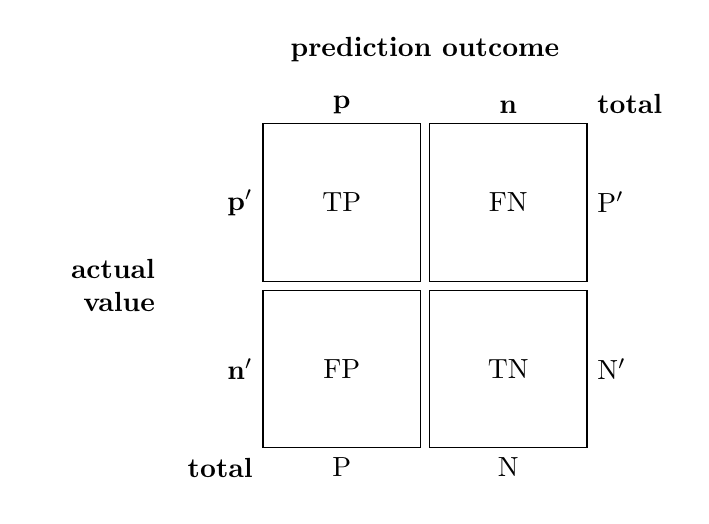
\begin{tikzpicture}[
        box/.style={draw,rectangle,minimum size=2cm,text width=1.5cm,align=right}]
        \matrix (conmat) [row sep=.1cm,column sep=.1cm] {
        \node (tpos) [box,
            label=left:\( \mathbf{p'} \),
            label=above:\( \mathbf{p} \),
            align=center] {TP};
        &
        \node (fneg) [box,
            label=above:\textbf{n},
            label=above right:\textbf{total},
            label=right:\( \mathrm{P}' \),
            align=center]
            {FN};
        \\
        \node (fpos) [box,
            label=left:\( \mathbf{n'} \),
            label=below left:\textbf{total},
            label=below:P,
            align=center] {FP};
        &
        \node (tneg) [box,
            label=right:\( \mathrm{N}' \),
            label=below:N,
            align=center] {TN};
        \\
        };
        \node [left=.05cm of conmat, text width=1.5cm,align=right] {\textbf{actual \\ value}};
        \node [above=.05cm of conmat] {\textbf{prediction outcome}};
    \end{tikzpicture}
\end{center}
And on this matrix we can compute several different metrics:
\begin{itemize}
    \item \textbf{Accuracy:} Represents the fraction of correctly labelled instances over the total number of instances.
    \begin{equation}
        Accuracy = \frac{TP + TN}{TP + TN + FP + FN}
    \end{equation}
    \item \textbf{Precision:} Represents the fraction of items labelled as positive that are actually positive. The higher the Precision, the lower the FPs.
    \begin{equation}
        Precision = \frac{TP}{TP + FP}
    \end{equation}
    \item \textbf{Recall:} Represents the fraction of positive items labelled as positive. The higher the Recall, the lower the FNs.
    \begin{equation}
        Recall = \frac{TP}{TP + FN}
    \end{equation}
    \item \textbf{F1-score:} combination of Precision and Recall to better ignore the biases of the precision and recall: the higher the F1-score, the lower FPs and FNs.
    \begin{equation}
        F1\-score = \frac{2 \cdot P \cdot R}{P + R}
    \end{equation}
    \item \textbf{True Positive Rate (TPR):} Represents the ability to correctly identify the elements of the positive class:
    \begin{equation}
    \label{eq:tpr}
        TPR = \frac{TP}{TP + FN}
    \end{equation}
    \item \textbf{True Negative Rate (TNR):} Represents the probability to correctly identify the elements of the negative class:
    \begin{equation}
    \label{eq:tnr}
        TNR = \frac{TN}{TN + FP}
    \end{equation}
\end{itemize}

\paragraph{}
Usually classifiers models outputs a score, a sort of probability to belong to one of the two class; this is also our case. Thus, there is the need of introducing a "cutting-off" threshold, which says at which value samples are classified as positive. For example, the basic threshold is set at $0.5$, thus all samples with a $score < 0.5$ are labelled as positive and all samples with a score $score >= 0.5$ are labelled as negative. \newline
Depending on the problem and on the requirements of the model, there can be the necessity to modify the threshold. Indeed, using a near one threshold we have a pessimistic classifier, with high Precision (few FPs) and low Recall (many FNs); using a near zero threshold, instead, we have an optimistic classifier since the Precision will be low (high false positive, everything is positive) and the Recall will be high (few false negatives).

\subsection{Receiver Operating Characteristic curve}
The ROC curve is another curve that we can generate to analyze how model's performances change as the threshold changes. It plots the TPR (equation \ref{eq:tpr}) against the TNR (equation \ref{eq:tnr}) and each point of the curve identifies a different classifier, in our case different "versions" of the same model. \newline
The ideal classifier would have $TPR = 1$ and $TNR = 0$, so would be located at the point $(0, 1)$; if the classifier always outputs the \textbf{positive class}, it would be located at $(1, 1)$ while if it always predicts the \textbf{negative class}, it is located at $(0, 0)$. We can also compare the algorithm with the random-guessing model\footnote{A very simple model that outputs a random score. It is used as a baseline for classifier models.}, since its performances are on the diagonal line. \newline
The random-guessing model will have a ROC AUC of $0.5$, thus every expert model are likely to have a greater AUC; if it is smaller, predictions must be flipped, e.g. if an instance is labeled as positive it should be changed as negative and the other way round.

\begin{figure}[hb]
    \centering
    \includesvg[width=0.6\textwidth]{Images/background/roc_curve.svg}
    \caption{An example of a Receiver Operating Characteristic curve, showing both the ideal curve and the curve from a generic model, with good results.}
\end{figure}
\newpage

\chapter{Related Work}
\label{ch:state_of_art}
\paragraph{}
\textbf{Anomaly Detection} refers to the problem of finding patterns in data that do not conform to expected behavior. 
This is a well-known problem in the literature and a lot of work has been done in this field since the end of the eighties. 

\paragraph{}
Generally speaking, there are three broad categories of anomaly detection algorithms, all based on the type of learning. Indeed, we can find anomaly detection exploiting \textit{supervised learning}, \textit{semi-supervised learning} and \textit{unsupervised learning}.
In particular,
\begin{itemize}
    \item \textbf{Supervised learning} means that all the instances of the dataset have a label indicating if the instance is anomalous or not. Algorithms of this kind are trained as two (or one)-class classifiers, such as \textit{One-Class SVM} \cite{one-class-svm}.
    
    \item \textbf{Semi-supervised learning} means that only a portion of data is labelled, that can be a subset of both inliers and outliers or only of one of them. It can also mean that we only have samples of the inliers and we train an algorithm on those; then, we can use the same algorithm to discriminize between inliers and outliers. One example of the latter technique are Auto-Encoders for computer vision, in which we train an Auto-Encoder to replicate the normal images and then we measure how much an instance is probably an outlier depending on the reconstruction error.
    
    \item \textbf{Unsupervised learning} means that we do not have labels at all, but only data instances. This is the most commonly used due to their wider and relevant application.
\end{itemize}

\paragraph{}
Another possible taxonomy of anomaly detection algorithms envisages three main categories: \textit{distance-based}, \textit{density-based} and \textit{model-based}. The first two categories are quite similar, because they define a measure of outlierness based on the number of neighboring points for each point, considered in the space of input vectors.
The three categories can be summarized as follows:
\begin{itemize}
    \item \textbf{Distance-based} methods compute, for each point $\textbf{p} \in \mathcal{D}$ in the dataset, the number of points inside the neighboring of radius $\varepsilon$ around this point; the set of neighbors is composed as $Neigh(\textbf{p}) = \{\ \textbf{q} \in \mathcal{D}\ |\ distance(\textbf{p}, \textbf{q}) < \varepsilon\ \}$. If this number is below a certain threshold, the point is considered as anomalous. \newline
    An example of algorithm belonging to this family is \textit{K-Nearest Neighbors} \cite{knn}.
    
    \item \textbf{Density-based} methods instead compute the density for each point $\textbf{p}$ as the fraction of points in the k-neighborhood of $\textbf{p}$ with respect the density around other points. In particular, a point is considered \textbf{inlier} if the density around the point is similar to the density around its \textit{k-neighbors}, while the point is considered as an \textbf{outlier} if the density around the point is significantly different from the local density of its \textit{k-neighbors}. \newline
    An example of algorithm belonging to this family is \textit{LOF} (\ref{sec:lof}) \cite{lof}.
    
    \item \textbf{Reconstruction-based} methods usually employ Neural Networks, training them to reconstruct the normal instances minimizing the reconstruction error \cite{ae_reconstruction}. The anomaly score is then computed as the reconstruction error: the higher it is, the higher the probability of being an anomaly.
    
    \item \textbf{Model-based} methods assume that inlier data points are generated from a model, thus the anomaly score is computed as the degree of deviation of the point from the model. The more an instance deviates from the model, the higher its probability to be an outlier. This methods try to fit some models on the data and then measure the deviation of the points from this fitted models. \newline
    Examples of this approach are classification based methods \cite{ad_classific} and clustering based methods \cite{clustering_based_ad}.
    Other examples of algorithms belonging to this family are Isolation Forest (iFor) \cite{ifor}, that builds an ensemble of Random Trees to isolate outliers, and Preference Isolation Forest (PIF) \cite{pif}, from which we take inspiration.

\end{itemize}

\paragraph{}
In the following we will analyze more in depth the algorithms that we will use for our comparisons in the results part, i.e. LOF, Isolation Forest and Preference Isolation Forest, that extends Isolation Forest. \newline
We choose those algorithms because we want to show that in the context of structured datasets, the density as used in LOF or iFor is not informative because the patterns can have different densities or anomalies can be found in high density regions even if they are not following any pattern. PIF has been chosen because it is our starting point and because we want to show the goal of our Thesis, that is building general models without any assumption on the nature of the patterns.

\section{Local Outliers Factor}
\label{sec:lof}
\paragraph{}
As already said, this algorithm belongs to the density-based family. In order to define what is the local density of a point, we need to introduce some concepts. \newline
First of all, we can introduce the notion of \textbf{k-distance} of a point $\textbf{p} \in \mathcal{D}$ in a dataset as the distance $distance(\textbf{p}, \textbf{q})$ between $\textbf{p}$ and $\textbf{q} \in \mathcal{D}$ such that, for any $k \in \mathbb{N}$:
\begin{enumerate}[label=(\roman*)]
    \item for at least $k$ objects $\textbf{q}' \in \mathcal{D} \backslash \{\textbf{p}\}$ it holds that $distance(\textbf{p}, \textbf{q}') \leq distance(\textbf{p}, \textbf{q})$, and
    \item for at most $k-1$ objects $\textbf{q}' \in \mathcal{D} \backslash \{\textbf{p}\}$ it holds that $distance(\textbf{p}, \textbf{q}') < distance(\textbf{p}, \textbf{q})$
\end{enumerate}
Then, we can define the \textit{k-distance neighborhood}, $N_k(\textbf{p})$, of an object $\textbf{p}$ as the set of points whose distance from $\textbf{p}$ is not greater than the \textit{k-distance}, i.e. 
\begin{equation}
    N_k(\textbf{p}) = N_{\textit{k-distance}(\textbf{p})}(\textbf{p}) = \{\ \textbf{q} \in \mathcal{D} \backslash \{\textbf{p}\}\ |\ distance(\textbf{p}, \textbf{q}) \leq \textit{k-distance}(\textbf{p}, \textbf{q})\ \}
\end{equation}

We can now introduce the notion of \textit{reachability-distance} of an object $\textbf{p}$ with respect to object $\textbf{o}$ as:
\begin{equation}
    \textit{reach-dist}_k(\textbf{p}, \textbf{o}) = max\ \{\ \textit{k-distance}(\textbf{o}), distance(\textbf{o}, \textbf{p})\ \}
\end{equation}

\begin{figure}[b]
    \centering
    \includesvg{Images/state_of_art/lof_kdist.svg}
    \caption{\textit{reach-dist}($\textbf{p}_1$, $\textbf{o}$) and \textit{reach-dist}($\textbf{p}_2$, $\textbf{o}$) for $k=4$}
    \label{fig:lof_kdist}
\end{figure}

This distance is equal to the actual distance between object $\textbf{p}$ and object $\textbf{o}$ if the two are far enough, while when they are "sufficiently" close, the distance becomes the \textit{k-distance} of $\textbf{o}$. This is done because with the parameter $k$ we can control the smoothing effect of the statistical fluctuations of the $distance(\textbf{o}, \textbf{p})$. 

\paragraph{}
Usually, in other density-based algorithms, there are two parameters that define the notion of density:
\begin{enumerate}[label=(\roman*)]
    \item \textbf{MinPts} specifying a minimum number of objects
    \item \textbf{Volume} specifying the volume in which to compute outlierness
\end{enumerate}
These two parameters determine a density \textit{threshold} for the algorithm to operate: objects or regions are connected if their neighborhood densities exceed the given density threshold. \newline
In LOF, instead, only \textbf{MinPts} is needed and to determine the density in the neighborhood of object \textbf{p} it uses the values $\textit{reach-dist}_{MinPts}(\textbf{p}, \textbf{o})$, for $\textbf{o} \in N_{MinPts}(\textbf{p})$.

We can now compute the \textit{local reachability density} of a point \textbf{p} as
\begin{equation}
    lrd_{MinPts}(\textbf{p}) = \frac{1}{
    \displaystyle \left ( \frac{\sum\limits_{\textbf{o} \in N_{MinPts}(\textbf{p}) } \textit{reach-dist}_{MinPts}(\textbf{p}, \textbf{o})}
    {|N_{MinPts}(\textbf{p}) |} \right ) }
\end{equation}

Intuitively, the local reachability density of an object \textbf{p} is the inverse of the average reachability distance based on the \textit{MinPts}-nearest neighbors of \textbf{p}. This quantity can be $\infty$ if all the reachability distances sums up to 0, that can occur whene there are at least \textit{MinPts} duplicates of \textbf{p} in the dataset.

\paragraph{}
Finally, we can introduce the \textit{Local Outlier Factor} of an object \textbf{p} as:
\begin{equation}
    LOF_{MinPts}(\textbf{p}) = \frac
    {\displaystyle \sum\limits_{\textbf{o} \in N_{MinPts}(\textbf{p}) } 
        \frac{lrd_{MinPts}(\textbf{o})}{lrd_{MinPts}(\textbf{p})}
    }
    {|N_{MinPts}(\textbf{p})|}
\end{equation}
that captures the degree to which we call \textbf{p} an outlier. It is computed as the average of the ratio of the \textit{local reachability density} of \textbf{p} and those of \textbf{p}'s \textit{MinPts}-nearest neighbors. The lower the \textbf{p}'s \textit{local reachability density} is, and the higher the \textit{local reachability density} of \textbf{p}'s \textit{MinPts}-nearest neighbors are, the higher is the \textit{LOF} value of \textbf{p}.

\paragraph{}
In the paper it is demonstrated that the \textit{LOF} value of each point is bounded as follows:
\begin{equation}
    \frac{direct_{min}(\textbf{p})}{indirect_{max}(\textbf{p})}
    \leq
    LOF(\textbf{p})
    \leq
    \frac{direct_{max}(\textbf{p})}{indirect_{min}(\textbf{p})}
\end{equation}
where $direct_{min}(\textbf{p}) = min\ \{\ \textit{reach-dist}(\textbf{p}, \textbf{q})\ |\ \textbf{q} \in N_{MinPts}(\textbf{p})\ \}$ is the minimum reachability distance between \textbf{p} and a \textit{MinPts}-nearest neighbor of \textbf{p} and $direct_{max}(\textbf{p})$ the corresponding maximum; $indirect_{min}(\textbf{p}) = min\ \{\ \textit{reach-dist}(\textbf{q}, \textbf{o})\ |\ \textbf{q} \in N_{MinPts}(\textbf{p})\ \wedge\ \textbf{o} \in N_{MinPts}(\textbf{q})\ \ \}$ instead represents the minimum reachability distance between \textbf{q} and a \textit{MinPts}-nearest neighbor of \textbf{q} and $indirect_{max}(\textbf{p})$ the corresponding maximum.

\paragraph{}
Summing up, LOF is a very famous algorithm that is able to capture the relative degree of isolation between points. Before this algorithm, most of the methods for outliers detection consider being an outlier as a binary property. In this algorithm, instead, they give a \textit{degree} of outlierness based on the isolation of the points. When an object is deep inside a cluster, its LOF value is approximately 1, while for other objects there are upper and lower bounds based on the \textit{MinPts} parameter.

\section{Isolation Forest}
\label{sec:ifor}
\paragraph{}
This algorithm \cite{ifor} belongs to the family of \textit{model-based} algorithms. This algorithm suggests an alternative method that explicitly isolates anomalies instead of incorporating normal instances behavior, unlike most existing model-based approaches that construct a profile of normal instances and then identify as anomalies those points that do not conform to the normal behavior. 

\paragraph{}
The main idea of the algorithm is to build an \textbf{ensemble} of \textit{random trees} that recursively partition a subset of the dataset $\mathcal{D}$ and gives a score to each point $\textbf{p} \in \mathcal{D}$ based on the average path-length of the point in the ensemble. The depth in which we find a point determines how many partitions are required to isolate the point; ideally, if a point is easy to isolate it is in a less dense region or has some parameters significantly different from other points, so it is more probably an outlier. On the contrary, normal points usually are in denser regions and have attribute values similar to other points, so they are more difficult to isolate and they are more probably inliers.

\begin{figure}[h!]
     \centering
     \begin{subfigure}{0.49\textwidth}
         \centering
        \includesvg[width=\textwidth]{Images/state_of_art/ifor_normal.svg}
         \caption{Isolation of a normal point}
         \label{subfig:ifor-normal}
     \end{subfigure}
     \begin{subfigure}{0.49\textwidth}
         \centering
        \includesvg[width=\textwidth]{Images/state_of_art/ifor_anom.svg}
         \caption{Isolation of an anomaly}
         \label{subfig:ifor-anom}
     \end{subfigure}
     \caption{Two examples of how a point can be isolated. If it is a normal point, figure \ref{subfig:ifor-normal}, it is harder to isolate and more splits are required. If instead it is an anomaly, figure \ref{subfig:ifor-anom}, it is easier to isolate and less splits are required.}
     \label{fig:ifor_isol}
\end{figure}

\paragraph{}
The algorithm is divided in two phases: \textbf{training} and \textbf{testing}. In the former, we build the ensemble of trees that isolate points; in the latter, we compute the path-length of the points and so the anomaly score for each point. \newline
The only parameters needed by the algorithm are the sub-sampling size $\psi$ and the number of trees in the ensemble, \textit{t}; in the paper, values suggested for this parameters are $\psi = 256$ and $t = 100$.

\paragraph{}
In order to show how the algorithm works, we need to introduce some concepts. First of all, we said that this algorithm builds an \textbf{ensemble} of \textbf{random trees}; an ensemble is simply a collection of models that are used all together, in order to have a more accurate result. \newline
A random tree, instead, is a \textit{binary decision tree} that, for each \textit{test-node}, selects randomly an attribute and a value for the split. Let \textit{T} be a node of the tree; \textit{T} can be an external node with no child, or an internal-node with one test and exactly two daughter nodes, $(T_L, T_R)$. A test consists of an attribute $a$ and a split value $v$ such that the test $a < v$ divides data points in $T_L$ and $T_R$. \newline

Given a dataset of points $\mathcal{D} = \{\ \textbf{p}_1,\ ...,\ \textbf{p}_n\ \}$ with $n$ instances, to build an isolation tree (iTree), we recursively divide $\mathcal{D}$ by randomly selecting an attribute $a$ and a value $v$ until one of the following conditions are met:
\begin{enumerate}[label=(\roman*)]
    \item The tree reaches a height limit;
    \item $|\mathcal{D}| = 1$;
    \item all data in $\mathcal{D}$ have the same value.
\end{enumerate}
When the tree is fully grown, the number of nodes is $2n - 1$ and so the total memory requirement is bounded linearly to \textit{n}.

\paragraph{}
In order to give an \textit{outlierness score} to points, it is possible to use the average path-length of the point in the trees, scaled by some factor. We can define the \textit{path-length} of a point \textbf{p}, $h(\textbf{p})$, as the number of edges traversed in an iTree from the root node until an external node containing \textbf{p} is reached. To normalize the \textit{path-length} we can compute the average path-length as an unsuccessful search in a BST\footnote{Binary Search Tree}, since they are structurally equivalent to iTrees, that is:
\begin{equation}
\label{eq:ifor_score_ad}
    c(n) = 2H(n-1) - \frac{2(n - 1)}{n}
\end{equation}
where $H(i)$ is the harmonic number, estimated as $H(i) \approx \ln{(i)} + e$, where the second term is the \textit{Euler's constant}. \newline
Since $c(n)$ is the average of $h(\textbf{p})$ given $n$, we can compute the anomaly score as
\begin{equation}
    \label{eq:ifor_score}
    s(\textbf{p}, n) = 2^{\displaystyle - \frac{E(h(\textbf{p}))}{c(n)}}
\end{equation}
where $E(h(\textbf{p}))$ is the average of $h(\textbf{p})$ from a collection of iTrees. From equation (\ref{eq:ifor_score}) it is possible to notice that $s$ is monotonic to $h(\textbf{p})$:
\begin{table}[h!]
    \begin{tabular}{l l l l l}
        \quad & $\bullet$ & when $E(h(\textbf{p})) \to 0$, & $s \to 1$; & \textbf{p} is an anomaly \\
        \quad & $\bullet$ & when $E(h(\textbf{p})) \to n-1$, & $s \to 0$; & \textbf{p} is an inlier \\
        \quad & $\bullet$ & when $E(h(\textbf{p})) \to c(n)$, & $s \to 0.5$; & \textbf{p} ambiguous situation
    \end{tabular}
\end{table}

\paragraph{}
At this point, we can analyze more in depth the training and evaluation stages.

\subsection{Training stage}
In this stage, we build the iTrees by recursively partitioning the dataset, until instances are isolated or a specific height threshold is reached. In this case, the tree height limit $l$ is automatically set by the sub-sampling size $\psi:\ l = ceiling(\log_2 \psi)$; this value represents the average tree height and the rationale to limit the trees at this height is that we are only interested in data points that have shorter-than-average path lengths, as those points are more probable to be outliers. \newline
Moreover, in the paper is shown that building the ensemble on a sub-sampled dataset without replacement\footnote{Sampling means that you (randomly) select a sub-set of the original set. Without replacement means that samples in the sub-set are not statistically independent because once you have selected an object, you cannot select the same object again; in other words, the same object cannot be selected twice.} leads to better results with respect when the whole dataset is used. \newline
The algorithm of iForest is the following:

\begin{algorithm}[h!]
    \caption{$iForest(\mathcal{D},\ \psi,\ t)$}
    \label{alg:iFor}
    \textbf{Input:} $\mathcal{D} = \{\ \textbf{p}\ |\ \textbf{p} \in \mathbb{R}^m\ \}$, $\psi$, $t$\\
    \textbf{Output:} a set of $t$ iTrees
    \begin{algorithmic}[1]
    \State \textit{F} $\gets$ Initialize forest
    \State $l \gets ceiling(\log_2 \psi)$ \Comment{set height limit}
    \ForAll{$i \in [0,\ t]$}
        \State $\textbf{D'} \gets sample(\mathcal{D},\ \psi)$
        \State $F \gets F\ \cup\ iTree(\textbf{D'},\ 0,\ l)$
    \EndFor
    \State \Return $F$
    \end{algorithmic}
\end{algorithm}

\begin{algorithm}[h!]
    \caption{$iTree(\mathcal{D},\ e,\ l)$}
    \label{alg:iTree}
    \textbf{Input:} $\mathcal{D} = \{\ \textbf{p}\ |\ \textbf{p} \in \mathbb{R}^m\ \}$, $e$ - current tree height, $l$ - height limit \\
    \textbf{Output:} an iTree
    \begin{algorithmic}[1]
    \If{$e \geq l\ or\ |\mathcal{D}| \leq 1$}
    \State \Return $exNode\{\ Size \gets |\mathcal{D}|\ \}$
    \Else
        \State $A \gets $ list of attributes in $\mathcal{D}$
        \State $a \in A$ select random attribute
        \State $v \in [min(a),\ max(a)]$ select random split value
        \State $\mathcal{D}_L \gets filter(\mathcal{D},\ a < v)$
        \State $\mathcal{D}_R \gets filter(\mathcal{D},\ a \geq v)$
        \State \Return $inNode\{\ Left \gets iTree(\mathcal{D}_L,\ e+1,\ l),$ \\
            \quad \quad \quad \quad \quad \quad \quad \quad \quad\ $Right \gets iTree(\mathcal{D}_R,\ e+1,\ l),$ \\
            \quad \quad \quad \quad \quad \quad \quad \quad \quad\ $SplitAtt \gets a$ \\
            \quad \quad \quad \quad \quad \quad \quad \quad \quad\ $SplitValue \gets v \}$
    \EndIf
    \end{algorithmic}
\end{algorithm}

\subsection{Evaluation Stage}
In this stage, an anomaly score $s$ is derived from the expected path length, $E(h(\textbf{p}))$, for each point in the dataset $\textbf{p} \in \mathcal{D}$. Using \textit{PathLength} (\ref{alg:path_function}), a single path length $h(\textbf{p})$ is derived by counting the number of edges $e$ from the root node to an external node as instance \textbf{p} traverses through an iTree. When \textbf{p} is terminated at an external node with more than one single point, the return value is $e + c(Size)$, where the adjustment account for an unbuilt subtree beyond the tree height limit. \newline
After having calculated $h(\textbf{p})$ for each iTree in the ensemble, we can compute $s(\textbf{p},\ \psi)$ (\ref{eq:ifor_score}) with a complexity of $O(n \cdot t \cdot \log \psi)$, where $n = |\mathcal{D}|$.

\begin{algorithm}[h!]
    \caption{$PathLength(\textbf{p},\ T,\ e)$}
    \label{alg:path_function}
    \textbf{Input:} $\textbf{p} \in \mathcal{D}$, $T$ - an iTree, $e$ - current tree height \\
    \textbf{Output:} path length of \textbf{p}
    \begin{algorithmic}[1]
    \If{$T$ is an external node}
        \State \Return $e + c(T.size)$ \Comment{$c(\cdot)$ is defined in equation \ref{eq:ifor_score_ad}}
    \EndIf
    \State $a \gets T.splitValue$
    \If{$\textbf{p}_a < T.splitValue$}
        \State \Return $PathLength(\textbf{p},\ T.left,\ e+1)$
    \Else   \Comment{$\textbf{p}_a \geq T.splitValue$}
        \State \Return $PathLength(\textbf{p},\ T.right,\ e+1)$
    \EndIf
    \end{algorithmic}
\end{algorithm}

\paragraph{}
Summing up, this algorithm proposes a new \textit{model-based} solution to Anomaly Detection, by isolating instances rather than profiling normal instance. It exploits the property of outliers that are "few and different" and an iTree is able to isolate anomalies closer to the root of the tree, compared to normal points. Exploiting random decision trees, it is able to have both spatial and temporal linear complexities. \newline
When examined more closely, it can be noticed that in reality this algorithm is \textit{density-based}, because anomalies are found depending on their isolation level: if a point is in a high density region, it will be harder to isolate. On the contrary, if a point is in a less dense region, it will be easier to isolate; therefore, the concept of isolation is in reality based on the concept of density.

\section{Preference Isolation Forest}
\label{sec:pif}

Also this algorithm belongs to the \textit{model-based} family, considering the problem of anomaly detection in a \textit{pattern-recognition} setup, where anomalies are samples that deviate from certain structured patterns. As previously stated, this differs from other algorithms, such as \textit{density-based} ones, in that we try to forecast the models (or patterns) that produced normal data rather than using a statistical measure to determine the outlierness score. Although density-based algorithms, in which the model describing inliers is a pdf\footnote{Probability Density Function}, can be seen as a special case of these \textit{pattern-recognition} algorithms, density-based and model-based algorithms are traditionally treated separately in the literature because they use different algorithms and methodologies. 

\paragraph{}
Anomaly detection in this setting is very challenging, since anomalies cannot be directly removed without having identified each and every structure first, but at the same time anomalies hinder the identification of existing structures. For this reason, anomalies are often detected as a byproduct of a multi-structure estimation process, performed with robust model fitting algorithms, like e.g. RANSAC \cite{ransac}, J-Linkage \cite{j_linkage} or T-Linkage \cite{t_linkage}. Within this framework, the structures underlying normal data are first identified and then all those points that do not conform with them are labeled as anomalous.

\paragraph{}
\textbf{Random Sample Consensus}\footnote{RANSAC} tries to fit a model to a dataset with a significat percentage of gross errors in a robust way. It follows the idea that rather than usign as much of the data as possible to obtain a model from data, it uses as small an initial dataset as feasible and enlarges this set with consistent data when possible. For example, given the task of fitting a line or an arc of a circle to a set of \textit{two-dimensional} points, RANSAC would select respectively a set of two or three points, since two points are required to fit a line and three are required to fit a circle. \newline
More formally, we can state the basic RANSAC paradigm as follows: \newline
Given a model that requires a minimum of $n$ points to instantiate its free parameters, and a set of data points $\mathcal{D}$ such that the number of points in $\mathcal{D}$ is greater than $n$ ($|\mathcal{D}| \geq n$), randomly select a subset $S_1$ of $n$ data points from \textbf{P} and instantiate the model. Use then the instantiated model $M_1$ to determine the subset $S_1^*$ of points that are within some error tolerance of $M_1$. The set $S_1^*$ is called \textbf{consensus set} of $S_1$. \newline
If $|S_1^*| \geq t$, with $t$ a threshold that is a function of the estimate of the number of errors in $\mathcal{D}$, use $S_1^*$ to compute a new model $M_1^*$. \newline
If $|S_1^*| < t$, randomly select a new subset $S_2$ and repeat the above process. If, after some predetermined number of trials, no consensus set with $t$ or more members has been found, either solve the model with the largest consensus set found or terminate in failure. 

\paragraph{}
Exploiting this robust model-fitting methods, PIF detects anomalies among structures whose nature is described by a given parametric function of unknown parameters. In order to do this, data is embedded in a high dimensional space called \textit{preference space} and then performs anomaly detection in this space relying on \textit{Pi-Forest}, an efficient tree-based method exploiting Voronoi Tessellations.
Given a dataset $\mathcal{D}$ of \textit{m-dimensional} points, the anomaly score of a point $s(\textbf{p})$ is computed in two main steps:
\begin{enumerate}[label=(\roman*)]
    \item Embed the data in the preference space;
    \item Adopt a tree-based isolation approach to detect anomalies in the preference space.
\end{enumerate}
The entire algorithm is detailed in \ref{alg:pif}.

\begin{algorithm}[h!]
    \caption{$PIF$}
    \label{alg:pif}
    \textbf{Input:} $\textbf{p} \in \mathcal{D}$, $t$ - number of trees, $\psi$ - sub-sampling size, $b$ - branching factor \\
    \textbf{Output:} Anomaly scores $\{\ s_\psi(\mathcal{E}(\textbf{p}_i))\ \}_{i=1,\ ...,\ n}$
    \begin{algorithmic}[1]
        \State \textit{/* Preference embedding */}
        \State $M_k \gets \{\ \bm{\theta}_i \ \}_{i=1,\ ...,\ k}$ \Comment{Sample $k$ models from $\mathcal{D}$}
        \State $P \gets preferenceEmbedding(\mathcal{D},\ M_k) \in \mathbb{R}^{nk}$
        \State
        \State \textit{/* Train Preference Isolation Forest */}
        \State $F \gets \textit{PI-Forest}(P,\ t,\ \psi,\ b)$
        \State
        \State \textit{/* Scoring input data */}
        \ForAll{$i \in [1,\ |P|]$}
            \State $\textbf{h} \gets [0,\ ...,\ 0] \in \mathbb{R}^t$
            \ForAll{$j \in [1,\ t]$}
                \State $T \gets $ \textit{j-th} PI-Tree in $F$
                \State $[\textbf{h}]_j \gets \textit{pathLength}(\textbf{pr}_i, T, 0)$ 
            \EndFor
            \State $s_\psi(\textbf{p}_i) \gets 2^{- \frac{E(\textbf{h}(\textbf{p}_i))}{c(\psi)}}$
        \EndFor
        \State \Return $\{\ s_\psi(\textbf{p}_i) \ \}_{i=1,\ ...,\ n}$
    \end{algorithmic}
\end{algorithm}

\subsection{Preference Embedding}
\label{subsec:preference_embedding}
\paragraph{}
Preference embedding refers to the procedure in which we map each point $\textbf{p} \in \mathcal{D},\ \textbf{p} \in \mathbb{R}^m$ in a k-dimensional vector, having components in the interval $[0,\ 1]$, via a mapping $\mathcal{E}: \mathcal{D} \rightarrow [0,\ 1]^k$. The space $[0,\ 1]^k$ is called \textbf{preference space}. \newline
More precisely, the embedding depends on a family of models $\mathcal{F}$ parametric in \textbf{$\theta$}, a set of $k$ model instances $\{\ \bm{\theta}_i\ \}_{i=1,\ ...,\ k}$ and an estimate of the standard deviation of the noise affecting the data, $\sigma$. \newline
A sample $\textbf{p}_i \in \mathcal{D}$ is then embedded to a vector $\textbf{pr}_i = \mathcal{E}(\textbf{p}_i)$ whose \textit{j-th} component is defined as:
\begin{equation}
\label{eq:preference_embedding}
    \textbf{pr}_i = \begin{cases} 
                      \phi(\delta_{ij}) & \delta_{ij} \leq 3\sigma \\
                      0 & otherwise
                   \end{cases}
\end{equation}
where $\delta_{ij} = \mathcal{F}(\textbf{p}_i, \bm{\theta}_j)$ is the residual of $\textbf{p}_i$ from the model $\bm{\theta}_j$; in other words, it represents how much the point deviates from the model. It is possible to use different functions to compute the preference, but $\phi$ must be monotonically decreasing in $[0,\ ...,\ 1]$ and such that $\phi(0) = 1$. In the paper the authors chose a Gaussian function of the form $\phi(\delta) = e^{ -\frac{\delta^2}{\sigma}}$. \newline
To give an idea of what the preference matrix $P$ represents, we can say that the \textit{j-th} component of the preference vector $\textbf{pr}_i$, namely $[\textbf{pr}_i]_j$, is the preference that a model $\bm{\theta}_j$ expresses for point $\textbf{p}_i$: the closer the point $\textbf{p}_i$ to the model $\bm{\theta}_j$, the higher the preference. The embedding function $\mathcal{E}$ maps dataset $\mathcal{D}$ to the set of preference vectors:
\[
    P = \{\ \textbf{pr}_i = \mathcal{E}(\textbf{p}_i)\ |\ \textbf{p}_i \in \mathcal{D}\ \}
\]
which represents the image of $\mathcal{D}$ through the embedding $\mathcal{E}$. As already said, the pool of models $\{\ \bm{\theta}_i\ \}_{i=1,...,k}$ of $k$ models is built using a RANSAC-like strategy: at each step, a new model is built sampling from the whole dataset.

\paragraph{}
In order to measure the distance in this new space, one very useful metric is the \textit{Tanimoto Distance}\footnote{First cited in \cite{tanimoto}, it is a generalization of the Jaccard Distance. If all the elements of the two vectors are binary (can be only 0 or 1), the two distances are the same. They are not the same if the two vectors can also have discrete values between 0 and 1.}, because points conforming to the same structures share similar preferences, yielding low distances. On the contrary, outliers would result in null (or few) preferences to the majority of structures, thus resulting in sparse preference vectors that tend to have distance close to 1 with the majority of other samples. \newline
Given two samples $\textbf{pr}_i = \mathcal{E}(\textbf{p}_i)$ and $\textbf{pr}_j = \mathcal{E}(\textbf{p}_j)$, their Tanimoto distance is:
\begin{equation}
    \label{eq:tanimoto}
    \tau(\textbf{pr}_i, \textbf{pr}_j) = 1 - \frac{\langle \textbf{pr}_i, \textbf{pr}_j \rangle}{||\textbf{pr}_i||^2 + ||\textbf{pr}_j||^2 - \langle \textbf{pr}_i, \textbf{pr}_j \rangle}
\end{equation}

\subsection{Pi-Forest}

At this point, after having built the preference matrix, we can isolate instances in the new space to identify outliers. Since in this space the Euclidean Distance, used e.g. in Isolation Forest \ref{sec:ifor}, is not informative, the authors needed to introduce a new type of Decision Tree, called \textit{Pi-Tree}, based on \textit{Voronoi Tessellation} (\ref{sec:voronoi}) and \textit{Tanimoto Distance}. \newline
The construction of a Pi-Tree is described in algorithm \ref{alg:pitree} and starts from a single region corresponding to the whole space $[0,\ 1]^k$ that is then recursively split in $b$ sub-regions by randomly selecting $b$ seeds $\{\ \textbf{s}_i \ \}_{i=1,...,b} \subset P$. At this point, the dataset is partitioned into $b$ subsets $\mathcal{P} = \{\ P_i \ \}_{i=1,...,b}$ and in each $P_i \subset P$ there are the points that have $\textbf{s}_i$ as the closest seed, according to Tanimoto Distance. The number of seeds $b$ is the branching factor of the tree associated to the splitting process; the construction of the tree stops when it is not possible to further split a region (i.e., the number of points in the region is less than $b$) or the tree has reached a maximum height, set as $l = \log_b \psi$, where $\psi$ is the number of points used to build the tree. In figure \ref{fig:voronoi} is illustrated the splitting procedure of a Pi-Tree.

\begin{figure}[h!]
    \centering
    \includesvg[width=0.9\textwidth]{Images/state_of_art/voronoi.svg}
    \caption{Example of a Pi-Tree with branching factor $b = 3$ and height limit $l = 3$, built from a set of points in $\mathbb{R}^2$. Every region is recursively split in $b$ sub-regions and can be noted that the most isolated samples fall in leaves at lowest heights, such as \textit{a} and \textit{d} cells.}
    \label{fig:voronoi}
\end{figure}

\begin{algorithm}[h]
    \caption{\textit{Pi-Tree}}
    \label{alg:pitree}
    \textbf{Input:} $P$ - preference matrix, $e$ - current tree height, $l$ - height limit, $b$ - branching factor\\
    \textbf{Output:} A Pi-Tree
    \begin{algorithmic}[1]
        \If{$e \geq l$ or $|P| < b$}
            \State \Return \textit{exNode}{$Size \gets |P|$}
        \Else
            \State randomly select a set of $b$ seeds $\{\ \textbf{s}_i\ \}_{i=1,...,b} \subset P$
            \State $\mathcal{P} \gets voronoiPartition(P,\ \{\ \textbf{s}_i\ \}_{i=1,...,b})$
            \State \textit{chNodes} $\gets \emptyset$
            \ForAll{$i \in [1,\ b]$}
                \State \textit{chNodes} $\gets chNodes \cup \textit{Pi-Tree}(P_i,\ e+1,\ l,\ b)$
            \EndFor
            \State \Return \textit{inNode} \{
                                            $ChildNodes \gets chNodes$, \\
                \quad \quad \quad \quad \quad \quad \quad \quad \quad\ $SplitPoints \gets \{\ \textbf{s}_i\ \}_{i=1,...,b}$
            \}   
        \EndIf
    \end{algorithmic}
\end{algorithm}

\paragraph{}
As already said for Isolation Forest (\ref{sec:ifor}), the outlierness score of a point depends on the height of the tree in which lies the point. This height is directly related to its separability, so a lower height corresponds to points that are separable with few splits, while a higher height corresponds to points hard to separate, thus are less probable to be outliers. \newline
In order to decrease the random fluctuations of the results of the algorithm, it is possible to build an ensemble of models called \textit{Pi-Forest}. We can build $t$ Pi-Trees each trained on a subset $P' \subset P$ of the preference representations of the dataset $\mathcal{D}$; the sub-sampling factor is controlled by $\psi$. \newline
The procedure is detailed in algorithm \ref{alg:piforest}.

\begin{algorithm}[h]
    \caption{\textit{Pi-Forest}}
    \label{alg:piforest}
    \textbf{Input:} $P$ - preference matrix, $\psi$ - sub-sampling size, $t$ - number of trees, $b$ - branching factor\\
    \textbf{Output:} A set of $t$ Pi-Tree
    \begin{algorithmic}[1]
        \State $F \gets \emptyset$
        \State set height limit $l = \log_b \psi$
        \ForAll{$i \in [1,\ t]$}
            \State $P^{'} \gets subSample(P,\ \psi)$
            \State $F \gets F \union \textit{Pi-Tree}(P^{'},\ 0,\ l,\ b)$
        \EndFor
        \State \Return $F$
    \end{algorithmic}
\end{algorithm}

\subsection{Anomaly Score}
Anomaly scores are computed as in Isolation Forest and other tree-based isolation methods, like \cite{isolation_anomal} and \cite{novel_anomal_score}. With reference to Isolation Forest, in this framework to compute the anomaly scores of the points we need first to embed the points in the preference space, build the Pi-Forest and then pass each instance $\textbf{pr} \in P$ through all the Pi-Trees of the ensemble. The heights reached in every tree are computed and collected in a vector $\textbf{h}(\textbf{pr}) = [h_1(\textbf{pr}),\ ...,\ h_t(\textbf{pr})]$ and are used to compute the anomaly score $s_\psi$ of an element as in Isolation Forest:
\begin{equation}
    s_\psi(\textbf{pr}) = 2^{\displaystyle \left ( - \frac{E(\textbf{h}(\textbf{p}))}{c(\psi)} \right )}
\end{equation}
where $E(\textbf{h}(\textbf{pr}))$ is the mean value over the elements of $\textbf{h}(\textbf{pr})$ and $c(\psi)$ is an adjustment factor with the same role as in Isolation Forest, see equation \ref{eq:ifor_score_ad}. \newline
Also the heights of elements in the trees are computed with a function similar to \textit{PathLength} - algorithm \ref{alg:path_function} - in Isolation Forest, but adapted for the Voronoi Tessellation:

\begin{algorithm}[h]
    \caption{$PathLength$}
    \label{alg:pathlength_pif}
    \textbf{Input:} $\textbf{pr}$ - a sample, $T$ - a Pi-Tree, $e$ - current path length \\
    \textbf{Output:} Path length of \textbf{pr}
    \begin{algorithmic}[1]
        \If{$T \textit{is an external node}$}
            \State \Return $e + c(T.size)$
        \EndIf
        \State $childNode \gets voronoiLocate(\textbf{pr},\ T.splitPoints,\ T.childNodes)$
        \State \Return $PathLength(\textbf{pr},\ childNode,\ e+1)$
    \end{algorithmic}
\end{algorithm}

Also in this case, all the observations for the adjustment factor has already been discussed in Isolation Forest. Notice that when the branching factor $b = 2$, the adjustment factor becomes as in \ref{eq:ifor_score_ad}, but if $n = 1$ the adjustment is $0$ and if $n = 2$, the adjustment is $1$.

\paragraph{}
The complexity of building the Pi-Forest is $\mathcal{O}(\psi \cdot t \cdot b \cdot log_b \psi)$ and the scoring phase has a complexity of $\mathcal{O}(n \cdot t \cdot b \cdot log_b \psi)$, where $n = |\mathcal{D}|$; with respect to Isolation Forest there is an additional overhead due to the preference embedding $\mathcal{E}(\cdot)$.

\paragraph{}
Concluding, we can state that Preference Isolation Forest has two main advantages over other isolation-based anomaly detection tools, that are the \textit{so-called} preference trick and the Voronoi Tessellation. The former, allows to integrate useful information about normal data and to better characterize structure-less anomalies. The latter, instead, preserves the intrinsic distance of the preference space during the splitting process, since the Tanimoto Distance (\ref{eq:tanimoto}) is employed. \newline
In the paper have been conducted several experiments on datasets generated by some pattern, like a line or a circle; in the majority of the experiments, this method gets better results because is able to distinguish between model-generated points and anomalous points. Other methods, instead, has troubles in identifying the patterns that generated the data.
\newpage

% \chapter{Problem formulation}
\label{ch:problem_formulation}




\chapter{Proposed Method}
\label{ch:proposed_solution}

\paragraph{}
First, we must conceptually distinguish between two concepts: the models that produce the data and the estimated machine learning models. \textbf{Pattern} refers to the actual model that specifies the manifold on which the data is located; it can represent geometrical figures, such as lines, parables, and circles, as well as more intricate curves; rather, we will refer to \textbf{models} as those that are built from data using statistical and machine learning techniques.

\paragraph{}
The novel \textbf{model-based} algorithm presented in this thesis aims to address the shortcomings of current approaches, in particular extending PIF applying a reconstruction-based ensemble. In the case of structured anomalies the density-based and distance-based approaches do not work, because those concepts are uninformative. In the model-based approach, instead, PIF represents an interesting approach since uses the preference trick to embed the dataset into a new space and applies a kind of Isolation Forest on this new space. \newline
The preference trick, as explained in \ref{subsec:preference_embedding}, is a measure of the deviation of the point from the learned model. Thus, the trick is to generate a new space in which the more models have high preference (low deviation) for a point, the more that point is probably a normal point.

\paragraph{}
This approach is notable, but it assumes that the patterns in the dataset have a known shape and the algorithm cannot generalize if the pattern can not be, or it is too complex to be, expressed analytically. In order to build the preference representation, PIF samples a high number of models that try to express preferences towards normal points.  Therefore, if we use a model representing a line to search for the pattern, we will discover only patterns that are represented as a line. Yet, if we use circles we will find only patterns with a circular shape. 

\paragraph{}
Our approach tries to build more general models learned directly from data, which can take any shape; in this way, the model adapts to the shapes found in the dataset and do not forces the patterns to be as assumed. Is a similar, but actually different, solution to PIF, but in our approach the models automatically adapts depending on the manifolds in the dataset.

\section{Problem Formulation}
\label{sec:problem_formulation}

\paragraph{}
The \textbf{\textit{input}} data is a dataset $\mathcal{D}$ made of noisy points in a \textit{m-dimensional} space: $\mathcal{D} = \{ \textbf{p} + \eta | \textbf{p} \in \mathbb{R}^m \}$, where $\eta = [\eta_1, .., \eta_i, ..., \eta_m]$ and $\eta_i \approx \mathcal{N}(0,\ \sigma^2_i)$ represents the noise affecting the data. The noise is modeled as an additive Gaussian noise with zero mean and unknown variance, applied to each dimension of the input vector.

\paragraph{}
Data points are divided in two disjoint subsets, the \textbf{\textit{normal}} points and the \textbf{\textit{anomalous}} points: $\mathcal{D} = \mathcal{N} \cup \mathcal{A}$ with $\mathcal{A} \cap \mathcal{N} = \emptyset$, where $\mathcal{N}$ is the set of normal points and $\mathcal{A}$ is the set of anomalies. \newline
\textbf{Normal} points lies on a set of \textit{k} \textbf{manifolds} in the \textit{m-dimensional} space, $\mathcal{N} \subseteq \mathcal{M}_1 \cup ... \cup \mathcal{M}_k$; each manifold represents a generic parametric function $\mathcal{F}_{\theta_i}$, where $\theta_i$ represents the parameter vector of the \textit{i-th} manifold. In a noisy-free setup all normal points lie on the manifolds, so each point \textit{p} belonging to the \textit{i-th} manifold, must satisfy $\mathcal{F}_{\theta_i}(\textbf{p}) = 0$. Note that the \textit{i-th} manifold is represented by $\mathcal{F}_{\theta_i}(\textbf{p})$ and so it is composed as $\mathcal{M}_i = \{ \textbf{p} : \mathcal{F}_{\theta_i}(\textbf{p}) = 0 \}$. Since in our case the points are noisy, we can expect $\mathcal{F}_{\theta_i}(\textbf{p}) \approx 0\ \forall\ \textbf{p} \in \mathcal{M}_i$.  \newline
\textbf{Anomalous} points $\mathcal{A}$, instead, do not have a standard behaviour and so do not lie in any manifold; thus, they form a subset $\mathcal{A} \subset \mathcal{D}$ and we know that $\mathcal{A} \not\subseteq \mathcal{M}_1 \cup ... \cup \mathcal{M}_k$. An anomaly is an observation that deviates so much from other observations as to arouse suspicion that it was generated by a different mechanism.

\paragraph{}
The \textbf{\textit{output}} of the algorithm $\mathcal{S} = \{s(\textbf{p}) \in [0, 1]\ |\ \textbf{p} \in \mathcal{D}\}$ is an anomaly score for each point, $s:\ \mathcal{D} \to \mathbb{R}$, representing a sort of "probability" that the point is anomalous. Thus, the score of a point is higher for points that are more probable to be anomalous and lower for normal points: $s(a) \gg s(n)$ for all $a \in \mathcal{A}$ and $n \in \mathcal{N}$.
\newline
This task is quite challenging, since the total number of manifolds, their structure and the noise affecting the data are unknown. It is necessary to learn the parameters that govern the patterns directly from data, contaminated by the anomalies.

\section{Rationale}

\paragraph{}
Considering the problem of Anomaly Detection in a structured dataset, the approach presented in PIF represents a big change. Thanks to the preference trick we are able to embed points in a new space, representing how much the learned models express a preference for each point. \newline
The preference expressed by a model $\mathcal{G}_j$ for a point $\textbf{p}_i \in \mathcal{D}$ represents the inverse of the deviation of the point from the model. In practice, the more the point is near to its representation built by the model, the more the preference $[\textbf{pr}_i]_j$ is high. Therefore, the preference space reflects how much each point is fitted by each model. \newline
If we would know the true pattern that generated normal points, all normal points would have a very high preference - because the deviation from the pattern is relatively small - and all the anomalies would have a very low preference - because the deviation is higher.

\paragraph{}
Note that in the following we will use the terms \textit{preference space} and \textit{preference matrix} as synonyms, but in reality they are different: the preference \textit{matrix} refers to a particular pool of models, while the preference \textit{space} is the space in which data points are projected. As an example, if we build two different pools of models the preference matrices will be different, but the space in which the points are projected is the same.

\paragraph{}
The preference space allows us to isolate data points depending on how many models have expressed a high preference for the points, thus it is mandatory to be able to build a preference space that reflects the nature of the dataset. In order to do that, we need to build models that can understand which patterns governs the data and replicate them. \newline
This is where the \textbf{novelty} of the approach developed in this thesis comes in: we build a pool of non-linear Neural Networks that are able to extract meaningful and appropriate patterns from the dataset without any prior knowledge on the nature of this patterns, as opposed to the way it is done in PIF, in which we assume a specific pattern to search and use that model to build the preference matrix. We have studied two kinds of Neural Networks, the Auto-Encoders \cite{ae_paper} and the Self-Organizing-Maps \cite{som_paper}. Both this models are able to adapt their weights to create a \textit{lower-dimensional} representation of the dataset, being able to hold only important features; since the anomalies represent data outside the patterns, the Neural Networks are able to discard their information and rely only on normal points to build the pattern representation.

\paragraph{}
PIF assumes that the type of patterns found in the dataset is known; e.g., it is known that normal data are originated from a line or from a circle; consequently, PIF will use, respectively, a line and a circle as learners and therefore the preference matrix will depend on the preferences expressed by this models. \newline
Such assumption reduces the use cases of PIF, because especially in real-world cases it is rare that the normal behavior is expressed by such simple models. \newline
Our algorithm, instead, does not have that limiting assumptions, but exploits the fact that several little models are built and try to approximate the patterns using those models. We want to build more general models learned directly from data, which can take any shape; in this way, the model adapts to the shapes found in the dataset and do not forces the patterns to be as assumed. Is a similar, but actually different, solution to PIF, because in our approach the models automatically adapts depending on the manifolds in the dataset.

\paragraph{}
The \textbf{goal of this thesis} is to show that using an ensemble of non-linear models such as Neural networks, trained on a subset of the dataset, we are able to approximate the patterns. \newline
We build models of lower degree with respect to the patterns' degree that try to approximate the manifold locally. At first, we will use as models Linear Regression and very simple Neural Networks with Auto-Encoder structure, but then we will also explore more complex and different models, such as deeper and wider Auto-Encoders and Self Organizing Maps.

\section{Algorithm}
\label{sec:algorithm}
The algorithm we propose for Anomaly Detection in structured normal data contaminated with high percentage of anomalies is structured similarly as PIF algorithm \ref{alg:pif}. It is composed of four main phases, that are listed below. The algorithm is shown in \ref{alg:npif}.

\begin{itemize}
    \item \textbf{Model building}: (lines 1-3) build the pool of models and train each model on a subset of the dataset, $\mathcal{MSS} \subset \mathcal{D}$, called \textbf{Minimum Sample Set} and has \textbf{cardinality} $\rho$, i.e. $|\mathcal{MSS}| = \rho$. This subset has the same role as in PIF, with the difference that in this case it represents the data instances on which train each model, while in PIF it represents the minimum samples needed to instantiate a model, e.g. two or three points are needed to instantiate respectively a line or a circle.
    
    \item \textbf{Preference Embedding}: (lines 5-18) embed each point into the preference space, generating the preference matrix $P \in \mathbb{R}^{N \times k}$ with $|\mathcal{D}| = N$ and $k$ the number of models. The value of element $(i, j)$ depends on the preference expressed by model $\mathcal{G}_j$ for point $\textbf{p}_i$, noted as $\delta_{ij}$.
    
    \item \textbf{Isolation Voronoi Forest}: (lines 20-21) apply the iVor (\ref{alg:piforest}) on the generated preference matrix, building the isolation forest made of Pi-Trees (\ref{alg:pitree}) on which compute the score.
    
    \item \textbf{Score computation}: (lines 23-30) compute the path length of each instance in each tree and finally compute the score, averaging between the computed path lengths and scaling by $c(\psi)$, refer to \ref{eq:ifor_score_ad}.
    
\end{itemize}

\begin{algorithm}[h!]
    \caption{\textit{Neural-PIF}}
    \label{alg:npif}
    \textbf{Input:} $\mathcal{D}$ - dataset, $k$ - number of models, $\rho$ - $\mathcal{MSS}$ size, $\tau$ - threshold,  $t$ - number of trees, $\psi$ - sub-sampling size, $b$ - branching factor \\
    \textbf{Output:} Anomaly scores $\{\ s_\psi(\mathcal{E}(\textbf{p}_i))\ \}_{i=1, ..., n}$
    \begin{algorithmic}[1]
        \State\textit{/* Build models */}
        \State $\mathcal{MSS} \in \mathbb{R}^{N \times \rho} \gets$ \textit{uniformSampling}($\mathcal{D}$, $\rho$)
        \Comment{Sample the Minimum Sample Sets, one for each instance $n \in N$, of size $\rho$}
        \State $\mathcal{M}_k \gets buildModels(\mathcal{D}, k, \rho)$
        \State
        \State \textit{/* Preference embedding $\mathcal{E}$ */}
        % \State $P \gets preferenceEmbedding(\mathcal{D},\ \mathcal{M}_k, \tau) \in \mathbb{R}^{nk}$
        \State $P \in \mathbb{R}^{nk}$ \Comment{initialize matrix}
        \ForAll{$i \in [0, n]$}
            \State $\textbf{p}_i \gets $ \textit{i-th} point of dataset
            \ForAll{$j \in [0, k]$}
                \State $\hat{\textbf{p}}_j \gets$ prediction of \textit{j-th} model for $\textbf{p}_i$
                \State $\delta_{ij} \gets$ distance between $\textbf{p}_i$ and $\hat{\textbf{p}}_i$
                \If{$\delta_{ij} \leq \tau$}
                    \State $P_{ij} \gets exp(-\delta_{ij} / \tau)$
                \Else
                    \State $P_{ij} \gets 0$
                \EndIf
            \EndFor
        \EndFor
        \State
        \State \textit{/* Train Preference Isolation Forest */}
        \State $F \gets \textit{PI-Forest}(P,\ t,\ \psi,\ b)$
        \State
        \State \textit{/* Scoring input data */}
        % \State $S_\psi(\mathcal{D}) \gets scoreDataset(P, F)\}$
        \ForAll{$i \in [1,\ |P|]$}
            \State $\textbf{h} \gets [0,\ ...,\ 0] \in \mathbb{R}^t$
            \ForAll{$j \in [1,\ t]$}
                \State $T \gets $ \textit{j-th} PI-Tree in $F$
                \State $[\textbf{h}]_j \gets \textit{pathLength}(\textbf{p}_i, T, 0)$
            \EndFor
            \State $s_\psi(\textbf{p}_i) \gets 2^{- \frac{E(\textbf{h}(\textbf{p}_i))}{c(\psi)}}$
        \EndFor
        \State \Return $s_\psi(\textbf{p}_i)_{i=1,\ ...,\ n}$
    \end{algorithmic}
\end{algorithm}

\section{Pattern learners}

In this section we will show different learners, that present different properties and capabilities in extracting the pattern from data. We will start with the most simple analytical models, like the Line and the Plane, showing that theoretically with an infinite number of those models it is possible to approximate a curve or a surface, respectively. \newline
Next, we will how it is possible to extract more complex patterns by employing more general models, like Auto-Encoders and Self-Organizing Maps.

\subsection{Line and Plane}
\paragraph{}
The first model from which to start is the most simple one, a straight line. It is known \cite{tangent_line_approx} that it is possible to linearly approximate all kind of curves at each point thanks to the tangent passing for that point. \newline
Given a function $y = f(x)$ that is differentiable at a point $p$, the function $f(\cdot)$ is locally linear and at the point $(p, f(p))$ can be approximated by its tangent. Thus, we can approximate the original function $f(\cdot)$ with a simpler function $L(\cdot)$ that is linear. We need to recall that when $f(x)$ is differentiable at $x = p$, the value of $f'(p)$ provides the slope of the tangent line to $y = f(x)$ at the point $(p, f(p))$. Therefore, the tangent line will have an explicit form like 
\begin{figure}[ht]
    \label{fig:linear_approx}
    \centering
    \includesvg[width=0.7\textwidth]{Images/problem_solution/linear_approx.svg}
    \caption{Example of a linear approximation on a generic function $y = f(x)$. In blue the true function, in green the tangent at the point $(p, f(p))$ that is marked in red.}
\end{figure}
\begin{equation}
    L(x) = f'(p)(x-p) + f(p)
\end{equation}
We will call $L(x)$ the \textit{first degree local linearization} of $f(x)$ at the point $(p, f(p))$ i.e. $L(x) \approx f(x)$ for $x \approx p$.

\paragraph{}
At this point we know that we can locally approximate any given function $f(\cdot)$ with a line, at each point; thus, ideally, with an infinite number of lines we can also derive the shape of the function. Starting from this idea, we would like to approximate any manifold with local approximations. In a \textit{two-dimensional} case, the linear approximation can be thought as a line; in a \textit{three-dimensional} case, the linear approximation is a plane.

\paragraph{}
In fact, considering a plane containing the point $\textbf{p} = (x_0, y_0, z_0)$ with a normal vector $\textbf{n} = \begin{bmatrix} a, & b, & c, \end{bmatrix}$, its equation is given by
\begin{equation}
    a(x - x_0) + b(y - y_0) + c(z - z_0) = 0.
\end{equation}
We know \cite{plane_local_approx} also that the gradient vector $\nabla f(x_0, y_0)$ is perpendicular to the level curve $f(x, y) = k$ at the point $\textbf{p}$; likewise, the gradient vector $\nabla f(x_0, y_0, z_0)$ is perpendicular to the level surface $f(x, y, z) = k$ at the point $\textbf{p}$. 

We should recall that the gradient vector is $\nabla f = \begin{bmatrix} \frac{\partial f}{\partial x}, & \frac{\partial f}{\partial y}, & \frac{\partial f}{\partial z} \end{bmatrix}$. Therefore, the tangent plane to the surface given by $f(x, y, z) = k$ at the point $\textbf{p}$, has the equation
\begin{equation}
    \frac{\partial f(x_0, y_0, z_0)}{\partial x}(x - x_0) + \frac{\partial f(x_0, y_0, z_0)}{\partial y}(y - y_0) + \frac{\partial f(x_0, y_0, z_0)}{\partial z}(z - z_0) = 0
\end{equation}

If we consider now a generic function of the form $z = f(x, y)$ and $F(x, y, z) = f(x, y) - z$ we can see that the surface given by $z = f(x, y)$ is identical to the surface given by $F(x, y, z) = 0$. The gradient of this function will be $\nabla F = \begin{bmatrix} \frac{\partial F}{\partial x}, & \frac{\partial F}{\partial y} & -1\end{bmatrix}$, because the last element is computed as $\frac{\partial }{\partial z}(f(x, y) - z)$. \newline
From the equation of the plane obtained above and solving for $z$, we obtain the local 2D approximation of a 3D surface:
\begin{equation}
    z = \frac{\partial f(x_0, y_0)}{\partial x}(x - x_0) + \frac{\partial f(x_0, y_0)}{\partial y}(y - y_0) + f(x_0, y_0)
\end{equation}

\begin{figure}[htb]
    \centering
    \includesvg[width=0.5\textwidth]{Images/problem_solution/local_plane.svg}
    \caption{Example of a plane, $\alpha$, the is tangent to the surface $f(x, y, z)$ at the point $\textbf{p}$.}
    \label{fig:local_plane}
\end{figure}

Therefore, our idea is to use the model line (or plane for the \textit{three-dimensional} space) not as the known pattern as in PIF, but as the model with which we can approximate any manifold. The algorithm using this model will function in the same way as in PIF when the pattern is a set of lines, but we show 
this procedure in this context in order to have a baseline to the next models, that should be able to locally approximate more complex functions and to better incorporate the patterns.

\subsection{Auto-encoders}
Auto-encoders (\ref{subsec:ae}) are a particular type of neural network whose structure consists of two parts: an encoder and a decoder. \newline
The \textit{encoder} tries to encode the input data, by reducing its dimensionality and creating the \textit{latent representation}. The \textit{decoder}, on the other hand, receives the latent representation and tries to reconstruct the original input. The trick that allows the network to \textbf{not} learn the identity matrix, which would be a copy of the original dataset, comes from the fact that the latent representation has fewer dimensions than the original input, thus it is forced to learn a representation of the input different from the identity. \newline
The output of the network and the training performed varies a lot depending on this factors:
\begin{enumerate}
    \item The \textbf{depth} of the network;
    \item The \textbf{width} of the network;
    \item The \textbf{activation} function of the layers. The major difference is between linear and non-linear activation functions: the latter allow the latent-space to be a non-linear transformation of the original input space and so allows to better capture the structure of the dataset.
\end{enumerate}

\begin{figure}[tb]
     \centering
     \begin{subfigure}[b]{0.3\textwidth}
         \centering
        \includesvg[width=\textwidth]{Images/problem_solution/autoencoders/dataset.svg}
         \caption{The dataset}
         \label{subfig:ds}
     \end{subfigure}
     \hfill
     \begin{subfigure}[b]{0.3\textwidth}
         \centering
        \includesvg[width=\textwidth]{Images/problem_solution/autoencoders/predictions_ae2.svg}
         \caption{MLP}
         \label{subfig:mlp}
     \end{subfigure}
     \hfill
     \begin{subfigure}[b]{0.3\textwidth}
         \centering
         \includesvg[width=\textwidth]{Images/problem_solution/autoencoders/predictions_ae1.svg}
         \caption{Auto-Encoder}
         \label{subfig:ae1}
     \end{subfigure}
     \caption{This figure shows the utility of the constraint on the latent representation's number of dimensions. In image \ref{subfig:mlp}, a Multi Layer Perceptron (MLP) network has learned to reconstruct the input vector generating a new vector in the same space; the problem is that this network didn't generate any latent representation with fewer dimension, thus it has learnt the identity matrix. On the contrary, in image \ref{subfig:ae1}, an Auto-Encoder with a latent representation with less dimensions than the input space has learned a new representation of the input dataset, not the identity matrix.}
     \label{fig:ae_constraint}
\end{figure}

Usually, as explained in \cite{ae_anom_detect}, auto-encoders for anomaly detection are trained on a dataset of normal instances that allow the network to understand the underlying pattern, being able to incorporate the patterns present in the normal instances. In the evaluation stage, the one in which an anomaly score is given to the instances, the score depends on the reconstruction error made by the network: the higher the error, the more probable the instance is anomalous. Indeed, since the network has incorporated the normal pattern, when the input is anomalous the reconstructed output will be very different from the input, while when the input is a normal point, the output of the network will be very similar to the original input. 

\paragraph{}
This method produces very good results, but it highly depends on the dataset used for training. In fact, it needs a human-labelled dataset in which normal points are separated from anomalies and the part of the dataset containing normal points should take in account all the possible behaviours that can be defined "normal"; if the set of normal points contains contaminations, the network will learn also the anomalous behaviour and if it is not highly representative of the normal behaviour, the model will produce many false negatives. \newline
The advantage is that it can be used to label single instances as normal or anomalous; indeed, once the network is trained it is possible to use it for any other instance of the same kind as the training data.

\paragraph{}
Our algorithm, instead, is able to train the pool of models directly on the \textbf{unlabelled} dataset, without the need for a separation between normal points and anomalies. Training the auto-encoders on a subset of the dataset allows each model to learn the pattern of a portion of the data and extract from it the normal behaviour. Using the preference trick, each model assigns a preference for its own "normal" instances using the learnt representation; in this way, we have several experts of some portion of the dataset and with Pi-Forest the algorithm can understand which instances are normal and which are not.

\paragraph{}
In the following sections we will show that an auto-encoder trained on a pure dataset, i.e. that does not contain anomalies, is able to learn the equation of a line or of a plane and the relationship between network's weights and coefficients of the pattern. \newline
This is crucial for our purposes, because it means that the auto-encoder is actually able to learn a useful representation of the pattern encoded, both in the encoder and in the decoder. Obviously this are examples showing the case in which the dataset is pure and the pattern is rather simple, but they nonetheless demonstrate the possibilities of an auto-encoder.

\subsubsection{Relationship between auto-encoders and lines}
\paragraph{}
Consider an auto-encoder with two input neurons, two output neurons, one hidden layer comprising one neuron and having the identity function $f(x) = x$ as activation. It will have four weights ($w_{02}, w_{12}, w_{23}, w_{24}$) and three biases ($b_{2}, b_{3}, b_{4}$).
\begin{figure}[ht]
    \centering
    \includesvg[width=0.7\textwidth]{Images/problem_solution/autoencoders/ae_212.svg}
    \caption{Structure of the network used in this section. The pedices of the weights are the starting neuron's index and the connected neuron's index. So, for example, weight $w_{02}$ goes from neuron $n_0$ to neuron $n_2$, or weight $w_{23}$ goes from neuron $n_2$ to neuron $n_3$. The biases have the same index to which they belong; for example, bias $b_4$ is the bias of neuron $n_4$.}
    \label{fig:ae_212}
\end{figure}
As we know, the output of a neuron is computed as the dot product of the weights and the input vector. Thus, the output of the hidden neuron can be computed as follows:
\begin{equation}
    h = w_{02} x + w_{12} y + b_2
\end{equation}
Therefore, the output of the network, $\hat{x}, \hat{y}$ is:
\begin{equation}
\label{eq:x_hat}
    \hat{x} = w_{23} \cdot h + b_{3}
\end{equation}
\begin{equation}
\label{eq:y_hat}
    \hat{y} = w_{24} \cdot h + b_{4}
\end{equation}
The goal of the network is to encode the input vector computing its latent representation and then decode the latent representation to reconstruct the input vector. It is trained to minimize the MSE (equation \ref{eq:MSE}), thus the error is computed calculating the euclidean distance between the prediction and the real point. Thus, the network must incorporate the data on which is trained to be able to replicate the same structure. \newline
Training this kind of network on a pure dataset in which the pattern is a line, we will show that exists a relationship between the weights and biases of the network and the coefficients of the pattern. Indeed, it is possible to compute those coefficients using the weights of the decoder part of the network.

\paragraph{}
From \cite{line_between_two_points} we know that given two points, $P_1 = \begin{bmatrix}x_1 & y_1\end{bmatrix}$ and $P_2 = \begin{bmatrix}x_2 & y_2\end{bmatrix}$, the line passing the two points is equal to the vector $P_2P_1$: 
$v_r = 
\begin{bmatrix}
    x_2 - x_1 \\
    y_2 - y_1
\end{bmatrix}$. Given the vector, we can write the vectorial equation of a line:
\begin{equation}
    \begin{bmatrix}
        x \\
        y
    \end{bmatrix}
    =
    \begin{bmatrix}
        x_1 \\
        y_1
    \end{bmatrix}
    + t \cdot \begin{bmatrix}
        x_2 - x_1 \\
        y_2 - y_1
    \end{bmatrix}
\end{equation}
Considering now a generic point $P$ belonging to the line, this forms a vector with respect to a point of the line, e.g. $P_1$:
\begin{equation}
    \overrightarrow{\rm P_1P} = P - P_1 = \begin{bmatrix}
        x - x_1 \\
        y - y_1
    \end{bmatrix}
\end{equation}
The vector $P_1P$ must be parallel and proportional to the vector $P_1P_2$, because it lies on the line equivalent to the vector $v_r$; thus, the vectors $P_1P$ and $P_1P_2$ must be linearly dependent and the equation of the line can be obtained solving the equation
\begin{equation}
    det \left ( 
    \begin{bmatrix}
        x - x_1 & x_2 - x_1 \\
        y - y_1 & y_2 - y_1
    \end{bmatrix}
    \right ) = 0
\end{equation}
that can be solved as follows:
\begin{equation}
    \begin{gathered}
        (x-x_1)(y_2-y_1) - (y-y_1)(x_2-x_1) = 0 \\
        xy_2 - x_1y_2 + x_1y_1 - yx_2 + yx_1 + y_1x_2 - y_1x_1 = 0 \\
        x_1y - x_2y - xy_1 + x_2y_1 + xy_2 - x_1y_2 = 0 \\
        y(x_1-x_2) + x(y_2 - y_1) -x_1y_2 + x_2y_1 = 0 \\
        y(x_1-x_2) = -(y_2-y_1)x + x_1y_2 - x_2y_1 \\
        y(x_1-x_2) = (y_1-y_2)x + x_1y_2 - x_2y_1 \\
        y = \frac{y_1-y_2}{x_1-x_2}x + \frac{x_1y_2 - x_2y_1}{x_1-x_2} \\
    \end{gathered}
\end{equation}
From this, we know that the slope of the line is $m = \frac{y_1-y_2}{x_1-x_2}$ and the intercept is $q = \frac{x_1y_2 - x_2y_1}{x_1-x_2}$.

\paragraph{}
Given two points $\hat{P}_1$ and $\hat{P}_2$ predicted by the network and using equations \ref{eq:x_hat} and \ref{eq:y_hat}, we can write the following:
\begin{equation}
    \begin{gathered}
        \hat{P_1} = \begin{bmatrix}
            \hat{x}_1 \\
            \hat{y}_1
        \end{bmatrix}
        = \begin{bmatrix}
            w_{23}h_1 + b_{3} \\
            w_{24}h_1 + b_{4}
        \end{bmatrix} \\
        \hat{P_2} = \begin{bmatrix}
            \hat{x}_2 \\
            \hat{y}_2
        \end{bmatrix}
        = \begin{bmatrix}
            w_{23}h_2 + b_{3} \\
            w_{24}h_2 + b_{4}
        \end{bmatrix}
    \end{gathered}
\end{equation}
where $h_1$ and $h_2$ are the hidden representations for the first and second point, respectively.
Substituting this values in the slope formula, we obtain the following result:
\begin{equation}
    \begin{gathered}
        m = \frac{\hat{y}_1 - \hat{y}_2}{\hat{x}_1 - \hat{x}_2} \\
        m = \frac{w_{24}h_1 + b_{4} - w_{24}h_2 - b_{4}}{w_{23}h_1 + b_{3} - w_{23}h_2 - b_{3}} \\
        m = \frac{w_{24}(h_1 - h_2)}{w_{23}(h_1 - h_2)} \\
        m = \frac{w_{24}}{w_{23}}
    \end{gathered}
\end{equation}
The same can be done with the equation of the intercept:
\begin{equation}
    \begin{gathered}
        q = \frac{\hat{x}_1\hat{y_2} - \hat{x}_2\hat{y}_1}{\hat{x}_1 - \hat{x}_2} \\
        q = \frac{(w_{23}h_1 + b_{3})(w_{24}h_2 + b_{4}) - (w_{23}h_2 + b_{3})(w_{24}h_1 + b_{4})}{w_{23}h_1 + b_{3} - w_{23}h_2 - b_{3}} \\
        q = \frac{w_{23}h_1b_{4} + w_{24}h_2b_{3} - w_{23}h_2b_{4} - w_{24}h_1b_{3}}{w_{23}(h_1 - h_2)} \\
        q = \frac{w_{24}b_{3}(h_2-h_1) + w_{23}b_{4}(h_1-h_2)}{w_{23}(h_1-h_2)} \\
        q = \frac{(h_1-h_2)(w_{23}b_{4} - w_{24}b_{3})}{w_{23}(h_1-h_2)} \\
        q = b_{4} - \frac{w_{24}}{w_{23}}b_{3}
    \end{gathered}
\end{equation}
At this point, we know that the network is able to encode the two input numbers in one number and then construct the equation of the line in the decoder. Indeed, we have shown that from the weights and the biases of the decoder is possible to reconstruct the equation of the line that generated the pattern.

\paragraph{}
One simple case that shows the correctness of this result is when the latent representation is equal to the $x$ coordinate of the input point. \newline
In this case, to compute the output for the $x$ coordinate is necessary to have $w_{23} = 1$ and $b_3 = 0$. Therefore, the slope of the line will be $m = \frac{w_{24}}{w_{23}} = \frac{w_{24}}{1} = w_{24}$ and the intercept will be $q = b_4 - 1 \cdot b_3 = b_4$. \newline
Thus, the $y$ coordinate of the input point is computed in the exact same way as is done when generating the pattern, because they are computed in the following way:
\begin{equation}
    \begin{gathered}
        y = m \cdot x + q \\
        \hat{y} = w_{24} \cdot h + b_4 = m \cdot x + q \quad if\ x = h\\
    \end{gathered}
\end{equation}

\subsubsection{Relationship between auto-encoders and planes}
\label{subsec:ae-planes}
\paragraph{}
Moving from the \textit{two-dimensional} to the \textit{three-dimensional} space, we want to show that the auto-encoder architecture is also able to incorporate the equation of a plane, that is the \textit{three-dimensional} "equivalent" of the line. \newline
In this case the network has a structure made of three input neurons, two neurons in the hidden layer and three neurons in the output layer. The \textit{three-dimensional} input vector is embedded in a \textit{two-dimensional} vector and then the original point will be reconstructed from the latent representation thanks to the decoder ability.

\paragraph{}
Similarly as we have done for the \textit{two-dimensional} case, we will define the network as follows: we have three input neurons, $n_0$, $n_1$, $n_2$ corresponding to the tree coordinate of an input point, two hidden neurons $n_3$ and $n_4$ and finally three output neurons, $n_5$, $n_6$, $n_7$, corresponding to the three coordinates of the predicted point.
\begin{figure}[ht]
    \centering
    \includesvg[width=0.7\textwidth]{Images/problem_solution/autoencoders/ae_323.svg}
    \caption{The structure of the network used in this section. The convention for naming the weights and biases is the same used in figure \ref{fig:ae_212}.}
    \label{fig:ae_323}
\end{figure}
Also in this case we can define the output of each neuron combining the weights entering the neuron and the biases. The hidden representation will be represented as a \textit{two-dimensional} vector, defined as follows:
\begin{equation}
    \begin{gathered}
        h = (h_3, h_4) \\
        h_3 = w_{03}x + w_{13}y + w_{23}z + b_3 \\
        h_4 = w_{04}x + w_{14}y + w_{24}z + b_4
    \end{gathered}
\end{equation}
The output values are instead computed as follows:
\begin{equation}
    \begin{gathered}
        \hat{x} = w_{35}h_3 + w_{45}h_4 + b_5 \\
        \hat{y} = w_{36}h_3 + w_{46}h_4 + b_6 \\
        \hat{z} = w_{37}h_3 + w_{47}h_4 + b_7
    \end{gathered}
\end{equation}
As already done for the line, we will show how it is possible to formulate the equation of a plane. At section \ref{sec:code_plane} there is the code with which we made the calculations to obtain the formulas. \newline
From \cite{plane_between_three_points} we know that the canonical equation of a plane is $ax + by + cz + d = 0$, where $a, b, c, d \in \mathbb{R}$ and $a, b, c$ are not simultaneously null. From Euclidean Geometry, we know that for three non-aligned points passes one and only one plane; thus, fixing an ortonormal cartesian reference system $RC(O, i, j, k)$, consider three non-aligned points:
\begin{equation}
    \begin{gathered}
        P_1 = (x_1, y_1, z_1) \\
        P_2 = (x_2, y_2, z_2) \\
        P_3 = (x_3, y_3, z_3)
    \end{gathered}
\end{equation}
Given that $P_1, P_2, P_3$ are not aligned, the vectors of each chosen couple, $\overrightarrow{P_1P_2}, \overrightarrow{P_1P_3}, \overrightarrow{P_2P_3}$ are linearly independent between them. If this is not the case, one couple will be linearly dependent and would be parallel, thus we would have three points lying on the same line. \newline
Considering a generic point $P = (x, y, z)$, will belong to the plane if and only if the vectors $\overrightarrow{P_1P}, \overrightarrow{P_1P_2}, \overrightarrow{P_1P_3}$ are coplanar. This is equivalent to ask that the determinant of the matrix having as rows the components of these vectors with respect to the base vector $(i, j, k)$ is null. \newline
We can rewrite the three vectors as following:
\begin{equation}
    \begin{gathered}
        \overrightarrow{P_1P} = P - P_1 = (x-x_1)i + (y-y_1)j + (z-z_1)k \\
        \overrightarrow{P_1P_2} = P_2 - P_1 = (x_2-x_1)i + (y_2-y_1)j + (z_2-z_1)k \\
        \overrightarrow{P_1P_3} = P_3 - P_1 = (x_3-x_1)i + (y_3-y_1)j + (z_3-z_1)k \\
    \end{gathered}
\end{equation}
Finally, we can say that the three vectors $\overrightarrow{P_1P}$, $\overrightarrow{P_1P_2}$ and $\overrightarrow{P_1P_3}$ are coplanars if and only if 
\begin{equation}
    det \left (\begin{bmatrix}
        x - x_1 & y - y_1 & z - z_1 \\
        x_2 - x_1 & y_2 - y_1 & z_2 - z_1 \\
        x_3 - x_1 & y_3 - y_1 & z_3 - z_1 \\
    \end{bmatrix} \right ) = 0
\end{equation}
Solving the equation with Laplace rules with respect to the first row, we get
\begin{equation}
    \label{eq:plane_estim}
    a(x - x_1) + b(y - y_1) + c(z - z_1) = 0
\end{equation}
where
\begin{equation}
    \label{eq:plane_coefficients}
    \begin{gathered}
        a = \ det \left (\begin{bmatrix}
            y_2 - y_1 & z_2 - z_1 \\
            y_3 - y_1 & z_3 - z_1 
        \end{bmatrix} \right ) \\
        b = - det \left (\begin{bmatrix}
            x_2 - x_1 & z_2 - z_1 \\
            x_3 - x_1 & z_3 - z_1
        \end{bmatrix} \right ) \\
        c = \ det \left (\begin{bmatrix}
            x_2 - x_1 & y_2 - y_1 \\
            x_3 - x_1 & y_3 - y_1
        \end{bmatrix} \right )
    \end{gathered}
\end{equation}
Rearranging equation \ref{eq:plane_estim} we get
\begin{equation}
    \begin{gathered}
        a(x - x_1) + b(y - y_1) + c(z - z_1) = 0 \\
        ax - ax_1 + by - by_1 + cz - cz_1 = 0 \\
        ax + by + cz - ax_1 - by_1 - cz_1 = 0
    \end{gathered}
\end{equation}
And with $d = -ax_1 - by_1 - cz_1$, we get the equation of the plane:
$ax + by + cz + d = 0$. From this, we can explicit the z-coordinate obtaining
\begin{equation}
    \label{eq:plane_z_explicit}
    z = -\frac{a}{c} x - \frac{b}{c} y - \frac{d}{c}
\end{equation}

\paragraph{}
At this point, we know how to compute the parameters of the equation of a plane given three points that are no coplanar. Our goal is to show that from the parameters of the neural network at figure \ref{fig:ae_323} it is possible to compute the equation of a plane, independent from the input point and the latent representation. \newline
As done in the case of the line, consider three points predicted from the network:
\begin{equation}
    \label{eq:ae_323_points}
    \begin{gathered}
        \hat{P_1} = \begin{bmatrix}
            \hat{x}_1 \\
            \hat{y}_1 \\
            \hat{z}_1
        \end{bmatrix}
        = \begin{bmatrix}
            w_{35}h_{3_1} + w_{45}h_{4_1} + b_{5} \\
            w_{36}h_{3_1} + w_{46}h_{4_1} + b_{6} \\
            w_{37}h_{3_1} + w_{47}h_{4_1} + b_{7} 
        \end{bmatrix} \\
        \hat{P_2} = \begin{bmatrix}
            \hat{x}_2 \\
            \hat{y}_2 \\
            \hat{z}_2
        \end{bmatrix}
        = \begin{bmatrix}
            w_{35}h_{3_2} + w_{45}h_{4_2} + b_{5} \\
            w_{36}h_{3_2} + w_{46}h_{4_2} + b_{6} \\
            w_{37}h_{3_2} + w_{47}h_{4_2} + b_{7} 
        \end{bmatrix} \\
        \hat{P_3} = \begin{bmatrix}
            \hat{x}_3 \\
            \hat{y}_3 \\
            \hat{z}_3
        \end{bmatrix}
        = \begin{bmatrix}
            w_{35}h_{3_3} + w_{45}h_{4_3} + b_{5} \\
            w_{36}h_{3_3} + w_{46}h_{4_3} + b_{6} \\
            w_{37}h_{3_3} + w_{47}h_{4_3} + b_{7} 
        \end{bmatrix}
    \end{gathered}
\end{equation}
Now, we can compute the coefficients of the plane substituting the three points in place of the generic coordinates, developing equation \ref{eq:plane_coefficients}:
\begin{equation}
    \begin{gathered}
        a = \hat{y}_{1} \hat{z}_{2} - \hat{y}_{1} \hat{z}_{3} - \hat{y}_{2} \hat{z}_{1} + \hat{y}_{2} \hat{z}_{3} + \hat{y}_{3} \hat{z}_{1} - \hat{y}_{3} \hat{z}_{2} \\
        b = - \hat{x}_{1} \hat{z}_{2} + \hat{x}_{1} \hat{z}_{3} + \hat{x}_{2} \hat{z}_{1} - \hat{x}_{2} \hat{z}_{3} - \hat{x}_{3} \hat{z}_{1} + \hat{x}_{3} \hat{z}_{2} \\
        c = \hat{x}_{1} \hat{y}_{2} - \hat{x}_{1} \hat{y}_{3} - \hat{x}_{2} \hat{y}_{1} + \hat{x}_{2} \hat{y}_{3} + \hat{x}_{3} \hat{y}_{1} - \hat{x}_{3} \hat{y}_{2} \\
        d = -a\hat{x}_1 - b\hat{y}_1 - c\hat{z}_1 = - \hat{x}_{1} \hat{y}_{2} \hat{z}_{3} + \hat{x}_{1} \hat{y}_{3} \hat{z}_{2} + \hat{x}_{2} \hat{y}_{1} \hat{z}_{3} - \hat{x}_{2} \hat{y}_{3} \hat{z}_{1} - \hat{x}_{3} \hat{y}_{1} \hat{z}_{2} + \hat{x}_{3} \hat{y}_{2} \hat{z}_{1}
    \end{gathered}
\end{equation}
For our calculations, we need also to compute the $-\frac{a}{c}$, $-\frac{b}{c}$ and $-\frac{d}{c}$ values, but we omit them for brevity.

\paragraph{}
The last step of our demonstration is to substitute the values of the various $\hat{x}$, $\hat{y}$ and $\hat{z}$ with the values of the points in \ref{eq:ae_323_points}. We get
\begin{equation}
    \begin{gathered}
        - \frac{a}{c} = \frac{- w_{36} w_{47} + w_{37} w_{46}}{w_{35} w_{46} - w_{36} w_{45}} \\
        - \frac{b}{c} = \frac{w_{35} w_{47} - w_{37} w_{45}}{w_{35} w_{46} - w_{36} w_{45}} \\
        - \frac{d}{c} = \frac{b_{5} w_{36} w_{47} - b_{5} w_{37} w_{46} - b_{6} w_{35} w_{47} + b_{6} w_{37} w_{45} + b_{7} w_{35} w_{46} - b_{7} w_{36} w_{45}}{w_{35} w_{46} - w_{36} w_{45}} = \\
        \quad\quad = b_7 - b_5 \left (\frac{- w_{36} w_{47} + w_{37} w_{46}}{w_{35} w_{46} - w_{36} w_{45}} \right ) - b_6 \left (\frac{w_{35} w_{47} - w_{37} w_{45}}{w_{35} w_{46} - w_{36} w_{45}} \right ) = \\
        \quad\quad = b_7 + \frac{a}{c} \cdot b_5 + \frac{b}{c} \cdot b_6
    \end{gathered}
\end{equation}

\paragraph{}
This equations show that an auto-encoder structured in this form is able to reconstruct a 3D point belonging to a plane from its 2D latent representation. In the decoder we have all the ingredients to incorporate the equation of the plane and to generate new points belonging to it. \newline
The entire network works in the training stage learns how to reproduce the input points, until it converges and the equation of the plane is encoded in the weights of the decoder part. At this point, we are able to generate 3D points belonging to the plane starting from 2D points generated e.g. from noise. 

\subsection{Self Organizing Maps}
\begin{figure}[hb]
     \centering
     \begin{subfigure}{0.4\textwidth}
         \centering
        \includesvg[width=\textwidth]{Images/problem_solution/som/MSS_som_line_before.svg}
         \caption{\textit{1D} before training}
         \label{subfig:som-one-before}
     \end{subfigure}
     \begin{subfigure}{0.4\textwidth}
         \centering
        \includesvg[width=\textwidth]{Images/problem_solution/som/MSS_som_line_after.svg}
         \caption{\textit{1D} after training}
         \label{subfig:som-one-after}
     \end{subfigure}
     \\
     \begin{subfigure}{0.4\textwidth}
         \centering
         \includesvg[width=\textwidth]{Images/problem_solution/som/MSS_som_square_before.svg}
         \caption{\textit{2D} before training}
         \label{subfig:som-two-before}
     \end{subfigure}
     \begin{subfigure}{0.4\textwidth}
         \centering
         \includesvg[width=\textwidth]{Images/problem_solution/som/MSS_som_square_after.svg}
         \caption{\textit{2D} after training}
         \label{subfig:som-two-after}
     \end{subfigure}
     \caption{Two examples of how SOM weights can be arranged. Red dots are weights in the input space, while the black lines are the connections between weights in the topology of the network. In plots \ref{subfig:som-one-before} and \ref{subfig:som-two-before} are shown the initial weights, representing also the arrangement of the weights matrix. Remember that in general, the displacement in the input space is different from the displacement in weight's matrix. In figures \ref{subfig:som-one-after} and \ref{subfig:som-two-after} show the displacement of the weights in the \textbf{input space} after the training procedure, that preserve the connections in the weights matrix.}
     \label{fig:som_weights}
\end{figure}

Self organizing maps (SOM) are a special kind of Neural Network used for unsupervised learning, to produce a \textit{low-dimensional} representation of a higher dimensional data set, preserving the topological structure of the data. \newline
This network is composed of two layers: one \textit{input} layer and one \textit{output} layer. The output layer is made of a set of weights $\mathcal{W} = \{\textbf{w}\ |\ \textbf{w} \in \mathbb{R}^m\}$, that are vectors in the same \textit{m-dimensional} space as the input vector $\textbf{p} \in \mathbb{R}^m$.
The set of weights can have different shapes, for example can be \textit{one-dimensional} and act like a line, or can be \textit{two-dimensional} with a grid or hexagonal displacement. \newline
The weights of this network lies in the same space as the input, so each weight represents a point in the space of the input vector, that is $\mathbb{R}^m$. At each iteration of the training procedure, the weights are update to become nearer to the input data: using competitive learning, the nearest weight to the input data and its neighbors are updated; after the training, the weights of the SOM will be placed near the most concentrated areas of the input data while preserving the topological structure of the weights. Indeed, weights that are neighbor in the network are also near in the \textit{m-dimensional} space.

\paragraph{}
What we need to know for our purposes is that this kind of model keeps an embedding of data in the weights, thus each weight $\textbf{w}$ is a representative of some samples in the dataset that have $\textbf{w}$ as the nearest weight. Therefore, the displacement of the weights both in the input space and in the topological space can be used to determine the patterns in the input dataset. \newline
\hspace{5pt} In figure \ref{fig:som_weights} can be seen two different SOMs trained on a $\mathcal{MSS}$ of size $\rho = 10$. In green there is the dataset, in red the weight's positions in the input space and the black lines are the connections between weights in the topology of the network. \newline
The first one is a SOM with a linear topology that represents a sort of line. After the training, the weights arranged in the input space moving towards denser regions, preserving the topology of the network thanks to the neighboring function \ref{eq:som_neighbor_func}. \newline
In the second one the SOM has a rectangular topology and the same effect can be noticed, allowing weights to fall in dense regions preserving the topology.

\section{Preference Embedding}
\paragraph{}
As said, the algorithm trains the pool of model, in which each learner is trained on a portion of the dataset and then the preference is computed. The preference in PIF paper is expressed as a function of the residual between a point and the model; in this thesis, instead, we consider the preference as a function of a quantity called \textbf{pseudo-preference} that depends on the model used, but as similarly as in the PIF's residual, therefore if a model express a low pseudo-preference for a point, the corresponding entry in the preference matrix will be higher, since is computed as a decreasing function of the pseudo-preference.

\paragraph{}
In particular, Auto-Encoders compute the preference as in PIF formulation, thus as the euclidean distance between the point and the prediction for that point. We choose this distance because is the same on which the network is trained, thus it represents the reconstruction error. Therefore, the preference of the Auto-Encoder $\mathcal{G}_j$ expressed for point $p_i$ is the following:
\begin{equation}
\label{eq:ae_preference}
    \delta_{ij} = (\textbf{p}_i - \hat{\textbf{p}}_i)^2
\end{equation}
where $\hat{\textbf{p}}_i = \mathcal{G}_j(\textbf{p}_i)$

\begin{figure}[hb]
     \centering
     \begin{subfigure}[b]{0.45\textwidth}
         \centering
        \includesvg[width=\textwidth]{Images/problem_solution/autoencoders/MSS_ae_after.svg}
         \caption{Set of predictions for the whole dataset, $\{ \mathcal{G}(\textbf{p}) | \textbf{p} \in \mathcal{D} \}$.}
         \label{subfig:ae_mss_preds}
     \end{subfigure}
     \hfill
     \begin{subfigure}[b]{0.45\textwidth}
         \centering
        \includesvg[width=\textwidth]{Images/problem_solution/autoencoders/MSS_ae_residuals.svg}
         \caption{Set of predictions for the whole dataset, $\{ \mathcal{G}(\textbf{p}) | \textbf{p} \in \mathcal{D} \}$.}
         \label{subfig:ae_mss_res}
     \end{subfigure}
     \caption{This figure shows the pseudo-preference expressed by an auto-encoder trained on a $\mathcal{MSS}$ of size $\rho = 10$. The higher the value (red), the lower the preference.}
     \label{fig:ae_residuals}
\end{figure}

\paragraph{}
Regarding Self Organizing Maps, however, express a meaningful preference from the network is not simple. We tried a lot of approaches, but we figured out that a method exploiting both the positions of the weight, i.e. position in the input space $\in \mathbb{R}^m$ and position in the topology of the weights set $\mathcal{W}$, could lead to better results. \newline
The process is composed of three steps:
\begin{enumerate}[label=(\roman*)]
    \item find, in the input space, the weight with minimum distance from $\textbf{p}$ among all the weights $\textbf{w} \in \mathcal{W}$;
    \item find the set of weights $\mathcal{Q} \subset \mathcal{W}$ that are neighbors to $\textbf{w}$ in the arrangement of $\mathcal{W}$;
    \item compute the preference for a point as the mean value of the distances between $\textbf{p}$ and $\mathcal{Q} \cup {\textbf{w}}$ in the input space.
\end{enumerate}
This computation takes advantage of the weights' natural arrangement in the network, whereby weights that are close together in the input space are likewise close together in the weights matrix's topology. Anomalies, on the other hand, are not defined by the pattern, therefore few weights will stay in its area. As a result, normal points that describe a pattern will have numerous weights in its neighborhood because during training weights were distributed there.

\begin{figure}[hb]
     \centering
     \begin{subfigure}[b]{0.45\textwidth}
         \centering
        \includesvg[width=\textwidth]{Images/problem_solution/som/MSS_som_line_residuals.svg}
         \caption{Linear SOM}
         \label{subfig:linear_som_res}
     \end{subfigure}
     \hfill
     \begin{subfigure}[b]{0.45\textwidth}
         \centering
        \includesvg[width=\textwidth]{Images/problem_solution/som/MSS_som_square_residuals.svg}
         \caption{Square SOM}
         \label{subfig:square_som_res}
     \end{subfigure}
     \caption{This figure shows the pseudo-preference expressed by two SOMs, one with a linear topology (fig \ref{subfig:linear_som_res}), the other with a square topology (fig \ref{subfig:square_som_res}). Both have been trained on a $\mathcal{MSS}$ of size $\rho = 10$. The higher the value (red), the lower the preference.}
     \label{fig:som_residuals}
\end{figure}

\paragraph{}
As an example, in figure \ref{fig:som_residuals} are shown the \textit{pseudo-preferences} expressed by the two SOMs of figure \ref{fig:som_weights} on the same dataset. The more an instance is towards the red color, the more it has high \textit{pseudo-preference} - and so smaller preference in the matrix. Therefore, the points belonging to the patterns have a smaller pseudo-preference and are more probably normal points.

\newpage

\chapter{Experiments}
\label{ch:experiments}
In this section we will show how we experimented our framework, analyzing the datasets used, the hyper-parameters of the framework, the testing procedure and finally commenting the results obtained with our framework, comparing our results with other State-Of-Art algorithms, like LOF and iFor.

\begin{figure}[htb]
     \centering
     \begin{subfigure}{0.17\textwidth}
         \centering
        \includesvg[width=\textwidth]{Images/datasets/ds_circle3.svg}
         \caption{Circle3}
         \label{subfig:circle3}
     \end{subfigure}
     \hfill
     \begin{subfigure}{0.17\textwidth}
         \centering
        \includesvg[width=\textwidth]{Images/datasets/ds_circle4.svg}
         \caption{Circle4}
         \label{subfig:circle4}
     \end{subfigure}
     \hfill
     \begin{subfigure}{0.17\textwidth}
         \centering
        \includesvg[width=\textwidth]{Images/datasets/ds_circle5.svg}
         \caption{Circle5}
         \label{subfig:circle5}
     \end{subfigure}
     \hfill
     \begin{subfigure}{0.17\textwidth}
         \centering
        \includesvg[width=\textwidth]{Images/datasets/ds_stair3.svg}
         \caption{Stair3}
         \label{subfig:stair3}
     \end{subfigure}
     \hfill
     \begin{subfigure}{0.17\textwidth}
         \centering
        \includesvg[width=\textwidth]{Images/datasets/ds_stair4.svg}
         \caption{Stair4}
         \label{subfig:stair4}
     \end{subfigure}
     \hfill
     \begin{subfigure}{0.17\textwidth}
         \centering
        \includesvg[width=\textwidth]{Images/datasets/ds_star5.svg}
         \caption{Star5}
         \label{subfig:star5}
     \end{subfigure}
     \hfill
     \begin{subfigure}{0.17\textwidth}
         \centering
        \includesvg[width=\textwidth]{Images/datasets/ds_star11.svg}
         \caption{Star11}
         \label{subfig:star11}
     \end{subfigure}
     \hfill
     \begin{subfigure}{0.17\textwidth}
         \centering
        \includesvg[width=\textwidth]{Images/datasets/ds_circles-parable3.svg}
         \caption{Parables}
         \label{subfig:circles-parable3}
     \end{subfigure}
     \hfill
     \begin{subfigure}{0.17\textwidth}
         \centering
        \includesvg[width=\textwidth]{Images/datasets/ds_lines-rects4.svg}
         \caption{Lines}
         \label{subfig:lines-rects4}
     \end{subfigure}
     \hfill
     \caption{List of all the 2D datasets used in the tests. Three of them contains circles, five contains lines and one contains parables.}
     \label{fig:all_datasets}
\end{figure}

\section{Data}
\hspace{5pt}
To validate our work, we experimented the algorithm on the same geometrical datasets used in PIF, that are synthetic 2D datasets describing different types of patterns. Moreover, we have generated other two 2D datasets and three 3D, containing four lines, three parables, one plane, one paraboloid and one sphere, respectively. \newline
The characteristics of the dataset are described in tables \ref{tab:syn_2d_ds_settings} and \ref{tab:syn_3d_ds_settings} and the 2D datasets can be visualized in figure \ref{fig:all_datasets}. \newline
In all the datasets the points are contaminated with random Gaussian noise and the anomalies are sampled uniformly in the ranges of the normal points. For each dataset, the number of anomalies is equal to the number of normal points, i.e. $|\mathcal{A}| = |\mathcal{N}|$. \newline
For each dataset, thanks to the available ground truth we were able to estimate the variance of the patterns. In particular, we estimated the variance of each pattern present in the dataset, e.g. in dataset \textit{star11} there are eleven patterns, and the dataset variance has been estimated as the mean value of the variances of each pattern $i \in [1, |\mathcal{M}|]$.

\begin{table}[h]
    \centering
    \resizebox{\textwidth}{!}{
        \begin{tabular}[width=\linewidth]{c  c  c  c  c  c}
        \hline
        \rowcolor{bluepoli!40}
             & |$\mathcal{D}$| & |$\mathcal{A}$| & |$\mathcal{N}$| & $E[\hat{\sigma}_{i=1,...,|\mathcal{M}|}]$ & |$\mathcal{M}_1$|, ..., |$\mathcal{M}_k$|  \\
        \hline
        circle3 & 1000 & 500 & 500 & 0.006 & $|\mathcal{M}_1| = 376$, $|\mathcal{M}_i| = 62$ $\forall i \in \{2, 3\}$ \\
        circle4 & 400 & 200 & 200 & 0.004 & $|\mathcal{M}_i| = 50$ $\forall i \in \{1, ..., 4\}$ \\
        circle5 & 500 & 250 & 250 & 0.003 & $|\mathcal{M}_i| = 50$ $\forall i \in \{1, ..., 5\}$ \\
        stair3 & 800 & 400 & 400 & 0.003 & $|\mathcal{M}_1| = 272$, $|\mathcal{M}_i| = 64$ $\forall i \in \{2, 3\}$ \\
        stair4 & 400 & 200 & 200 & 0.004 & $|\mathcal{M}_i| = 50$ $\forall i \in \{1, ..., 4\}$ \\
        star5 & 500 & 250 & 250 & 0.009 & $|\mathcal{M}_i| = 50$ $\forall i \in \{1, ..., 5\}$ \\
        star11 & 1100 & 550 & 550 & 0.005 & $|\mathcal{M}_i| = 50$ $\forall i \in \{1, ..., 11\}$ \\
        parables & 600 & 300 & 300 & 0.02 & $|\mathcal{M}_i| = 100$ $\forall i \in \{1, ..., 3\}$ \\
        lines & 800 & 400 & 400 & 0.02 & $|\mathcal{M}_i| = 100$ $\forall i \in \{1, ..., 4\}$ \\
        \hline
        \end{tabular}
    }
    \caption{Synthetic (2D) datasets settings}
    \label{tab:syn_2d_ds_settings}
\end{table}

\begin{table}[h]
    \centering
    \resizebox{\columnwidth}{!}{
        \begin{tabular}[width=\linewidth]{c  c  c  c  c  c}
        \hline
        \rowcolor{bluepoli!40}
             & |$\mathcal{D}$| & |$\mathcal{A}$| & |$\mathcal{N}$| & $\hat{\sigma}$ & |$\mathcal{M}_1$|, ..., |$\mathcal{M}_k$|  \\
        \hline
        plane & 1000 & 500 & 500 & 0.05 & $|\mathcal{M}| = 500$ \\
        
        paraboloid & 1000 & 500 & 0.05 & 500 & $|\mathcal{M}| = 500$ \\
        
        sphere & 1000 & 500 & 500 & 0.05 & $|\mathcal{M}| = 500$ \\
        \hline
        \end{tabular}
    }
    \caption{Synthetic (3D) datasets settings}
    \label{tab:syn_3d_ds_settings}
\end{table}


\section{Methodology}
\subsection{Hyper-parameters}
\paragraph{}
To be able to study the behavior of the algorithm in different scenarios, some hyper-parameters changes test by test while others remain stable. In the latter case we find the number of training epochs, the learning rate, the number of models used and the parameters of the Voronoi Forest built in the last phase of the algorithm; this ones are kept the same as suggested in PIF paper. \newline
In contrast, what changes depending on the experiment are the Minimum Sample Set Size $\rho$, determining the cardinality of the sub-set on which the models are trained, the architecture of the networks and most important the inlier threshold $\tau$, used for the preference embedding. Possible values of the parameters are listed in table \ref{tab:hyper-params} \newline

\begin{table}[h]
    \centering
    \resizebox{\textwidth}{!}{
        \begin{tabular}[width=\linewidth]{c  c}
        \hline
        \rowcolor{bluepoli!40}
             Hyper-parameter & Values \\
        \hline
        AE architecture 1 ($AE_1$) & (2, 4, 1, 4, 2) \\
        AE architecture 2 ($AE_2$) & (2, 8, 4, 1, 4, 8, 2) \\
        AE architecture 3 ($AE_3$) & (3, 5, 2, 5, 3) \\
        AE architecture 4 ($AE_4$) & (3, 9, 5, 2, 5, 9, 3) \\
        SOM architecture 1 ($SOM_1$) & (1, 10) \\
        SOM architecture 2 ($SOM_2$) & (5, 5) \\
        $\rho$ & [2, 5, 10, 20, 30, 100] \\
        $\tau$ & $[1, 4, 7, 10, 25, 50, 100] \cdot \sigma$ \\
        \hline
        training epochs & 500 \\
        n.o models & 2000 \\
        learning rate & 0.01 \\
        activation function & tanh($\cdot$) \\
        \hline
        \end{tabular}
    }
    \caption{Auto-Encoders architectures list the number of neurons in each layer. SOM architectures list the number of neurons as a tuple (num of rows, num of cols).}
    \label{tab:hyper-params}
\end{table}
We choose to keep only some of the hyper-parameters variables, because are the ones that have a higher impact on the performances of the dataset. First, the network's architecture determines how much the network is big and how it is arranged in the case of the SOM. Bigger networks have bigger potential because could learn more, but the number of data on which is trained ($\rho$) is the same; thus, its performances are not necessarily better, because the lack of data and the higher number of parameters to learn could not bring the network to convergence.

\paragraph{}
As said, $\rho$ determines the size of the sub-set on which networks are trained. Usually, Neural Networks need a high number of samples for training, because they have a high number of parameters compared to other methods; we decided to employ relatively small neural networks in order to have fewer parameters and a better training convergence since $\rho$ is relatively small. This choices leads to have smaller computational complexity, and follow the RANSAC's principle. \newline
Moreover, $\rho$ controls also the probability of sampling a \textit{pure} $\mathcal{MSS}$, i.e. a $\mathcal{MSS}$ that contains only normal points, without anomalies. Since we employed a randomized sampling, the probability of each point to be selected is $\frac{1}{N}$; therefore, with $\rho = 1$ we have $\frac{1}{2}$ probability of getting a pure $\mathcal{MSS}$. With $\rho = 2$, we have four possibilities of sampling, only one of which comprises both normal samples. Continuing, for each $\rho \in [1, N]$, we can say that the probability of getting at least one pure $\mathcal{MSS}$ is $\displaystyle \frac{1}{2^\rho}$. Therefore, with a higher $\rho$ we increase the number of samples on which each network is trained, but we also reduce the possibility of getting pure models, i.e. those models trained on pure $\mathcal{MSS}$.

\paragraph{}
Another important hyper-parameter is $\tau$, the \textit{inlier threshold}. This threshold, according to equation \ref{eq:preference_embedding}, determines if a point is considered normal, with its degree of "normality", or an anomaly, with a score of zero, for the current model. Therefore, a near-zero threshold would consider normal points only those that have a very low residual, while a high threshold allows more points to be considered normal. \newline
This threshold influences the values in the preference matrix, thus changing the functioning of the Isolation Voronoi Forest. Finding the good trade-off between the inlier threshold and accuracy of the model is not easy and a grid-search is required to reach the best performances depending on our requirements. 

\subsection{Testing Procedure}
\paragraph{}
The testing procedure has been structured hierarchically and we tested each possible combination comprising the dataset to use, the architecture, the threshold $\tau$ and the size of the sub-sampling set $\rho$. \newline
Therefore, the testing routine is structured as follows, where \textit{Neural-PIF} is detailed in algorithm \ref{alg:npif}:

\begin{algorithm}[h!]
    \caption{\textit{Testing procedure}}
    \label{alg:testing}
    \textbf{Input:} $\bm{\mathcal{D}}$ - the set of dataset, $\mathcal{G}$ - model to use, $\bm{\tau}$ - all possible values of the normal threshold,  $\bm{\rho}$ - all possible values of the sub-sampling size \\
    \begin{algorithmic}[1]
        \ForAll{$\mathcal{D} \in \bm{\mathcal{D}}$}
            \ForAll{$\tau \in \bm{\tau}$}
                \ForAll{$\rho \in \bm{\rho}$}
                    \State $scores = \textit{Neural-PIF}(\mathcal{D}, \tau, \rho, \mathcal{G})$
                    \State $AUC = \textit{computeROCauc}(scores)$
                \EndFor
            \EndFor
        \EndFor
    \end{algorithmic}
\end{algorithm}

After running all the experiments, we ended up with the ROC's AUC reached by each combination of parameters. In appendix \ref{app:appendix_b} there are the plots showing for each dataset and for each model how the AUC varies depending on $\tau$ and $\rho$.

\section{Results}
\subsection{Two-dimensional data}

\paragraph{}
In this section we will analyze the results obtained with each model, considering different combinations of the aforementioned hyper-parameters. \newline
In table \ref{tab:results-2d} there are the results reached by each of the presented model, plus two State Of Art algorithms' results. Results of LOF and iFor have been computed running one hundred experiments for each dataset and taking then the mean value, while PIF's results are taken from its paper. In appendix A in lists \ref{lst:lof_exp_code} and \ref{lst:ifor_exp_code}, we show the code to reproduce the above experiments. \newline
Results of the models presented in this thesis, instead, are taken as the maximum value reached for that specific architecture for that dataset; in other words, we took the maximum value independently of $\tau$ and $\rho$ from the plots in \ref{app:appendix_b}.

\begin{table}[hb]
    \centering
    \resizebox{\columnwidth}{!}{
        \begin{tabular}[width=\linewidth]{c c c c c c c c}
        \hline
        \rowcolor{bluepoli!40}
             Dataset & LOF & iFor & $AE_1$ & $AE_2$ & $SOM_1$ & $SOM_2$ & PIF \\
        \hline
        circle3              & 0.691 & 0.708 & 0.865 & 0.872 & 0.869 & \underline{0.874} & \textbf{0.930} \\
        circle4              & 0.610 & 0.633 & 0.656 & 0.689 & \underline{0.756} & 0.726 & \textbf{0.897} \\
        circle5              & 0.577 & 0.567 & 0.660 & 0.688 & 0.711 & \underline{0.725} & \textbf{0.780} \\
        stair3               & 0.717 & 0.940 & 0.968 & 0.972 & \underline{0.975} & \textbf{0.977} & 0.971 \\
        stair4               & 0.809 & 0.889 & \underline{\textbf{0.957}} & 0.950 & 0.955 & 0.956 & 0.952 \\
        star5                & 0.753 & 0.731 & 0.806 & 0.829 & 0.831 & \underline{0.850} & \textbf{0.910} \\
        star11               & 0.665 & 0.742 & 0.773 & \underline{0.775} & 0.760 & 0.768 & \textbf{0.796} \\
        \hline
        Mean$_{PIF}$           & 0.689 & 0.744 & 0.812 & 0.825 & 0.837 & \underline{0.839} & \textbf{0.891} \\
        \hline
        parables             & 0.838 & 0.813 & 0.907 & \underline{\textbf{0.920}} & 0.911 & 0.918 & - \\
        lines                & 0.809 & 0.818 & 0.914 & 0.913 & 0.914 & \underline{\textbf{0.916}} & - \\
        \hline
        Mean$_{TOT}$                 & 0.719 & 0.760 & 0.834 & 0.845 & 0.854 & \underline{\textbf{0.857}} & - \\
        \end{tabular}
    }
    \caption{Results on synthetic 2D datasets. Bold elements represent the higher value on the row. Underlined elements instead represents the maximum value on the row, but without considering PIF results.}
    \label{tab:results-2d}
\end{table}

We compared our algorithm, in four different variants, with LOF and iFor; PIF results are shown only as a benchmark and not as a comparision, because it would not be fair. Indeed, PIF has higher knowledge with respect our algorithm, because it assumes to know the correct pattern to search. Therefore, our algorithm lies in the middle between PIF and other density-based or model-based algorithms, because we exploit the preference trick and the structure of the dataset, but we are not as informed as in PIF. \newline
Therefore, we will make the comparisons by comparing only those algorithms that have the same dataset information as ours, i.e., none.

\paragraph{}
First of all, we will compare our algorithm in general with the two state-of-art competitors and then we will compare the different versions of our algorithm.

\paragraph{}
As can be noted from the table, LOF and iFor have much lower performances on this datasets, loosing up to $10\%$ over the mean AUC values. This is due to the fact that this algorithms do not try to understand how data is composed and arranged, i.e. learn the pattern, but rather computes the anomaly scores depending on the density of the point or considering how much the point is easy to isolate. \newline
Since in structured normal data dataset the density is not informative, this algorithms are not able to reach our algorithm's performances.

\paragraph{}
Considering instead our algorithm, we can notice that using SOMs as learners we reach higher performances. Both the models, AEs and SOMs, are able to learn a pattern and understand useful information from data, but the difference could be due to how the models learn and computes the preference. \newline
Auto-Encoders learn a hidden representation of the data and reconstruct original input vector, therefore are able to generate \textit{m-dimensional} vectors in all $\mathbb{R}^m$ and if we input an infinite number of vectors belonging to a continuous function to the auto-encoder, it will output a continuous function. Therefore, it is as if the auto-encoder learns a \textit{continuous} representation of the $\mathcal{MSS}$ on which it is trained.

\paragraph{}
On the contrary, SOMs during training moves a finite number of weights in the input space and at inference time it returns the weight closer to the input vector. Therefore, if we input to the SOM an infinite number of points belonging to a pattern, as we could do with the auto-encoder, as output we will get only a finite number of points defined by the weights of the network. \newline
Therefore, it is as if the SOM learns a \textit{discrete} representation of the $\mathcal{MSS}$ on which it is trained, because the possible outputs of the network are defined only where the weights are.

\paragraph{}
Analyzing this differences in the type of learning and inference performed by the two networks, it is clear why there is such difference in the results in the table. Since the datasets mostly contain several patterns and not only one, the union of all this patterns could be thinked as a unique non-continuous pattern. In this case, therefore, it is better to learn a discrete representation instead of a continuous one. Therefore, theoretically auto-encoders should perform better when the manifolds are continuous and smooth, while SOMs perform better when the manifolds are discontinuous and broken in pieces.

\subsection{Three-dimensional data}
\paragraph{}
In table \ref{tab:results-3d} are shown results for the same algorithms as in the \textit{two-dimensional} case, applied to synthetic datasets comprising a plane, a paraboloid and a sphere. In this case the results of PIF are not given, because in the paper it has not been tested on this datasets.

\begin{table}[h]
    \centering
    \resizebox{\columnwidth}{!}{
        \begin{tabular}[width=\linewidth]{c c c c c c c}
        \hline
        \rowcolor{bluepoli!40}
             Dataset & LOF & iFor & $AE_3$ & $AE_4$ & $SOM_1$ & $SOM_2$ \\
        \hline
            plane                & 0.827 & 0.725 & \textbf{0.940} & 0.936 & 0.897 & 0.899 \\
            paraboloid           & 0.690 & 0.591 & 0.878 & \textbf{0.906} & 0.845 & 0.845 \\
            sphere               & 0.651 & 0.783 & 0.828 & \textbf{0.858} & 0.789 & 0.771 \\
            \hline
            Mean                 & 0.722 & 0.699 & 0.882 & \textbf{0.900}  & 0.844 & 0.838 \\
            \hline
        \end{tabular}
    }
    \caption{Results on synthetic 3D datasets. Results in bold are the maximum value along the row.}
    \label{tab:results-3d}
\end{table}

\paragraph{}
In this situations, the comparison with the state-of-art algorithms is the same as in the \textit{two-dimensional} case, with the state-of-art algorithms loosing up to $20\%$ of ROC AUC. \newline
Again, this discrepancy can be explained by the fact that in the dataset all regions have more or less the same density, since anomalies have been sampled from a uniform distribution. Therefore, also in this case the density is not informative and the algorithms perform poorly.

\paragraph{}
This results also confirm another observation made for the \textit{two-dimensional} case, that is the fact that SOMs prefer discontinuous and non-smooth manifolds, while auto-encoders prefer continuous and smooth manifolds. Since in each of this dataset there was only one continuous and smooth manifold, the auto-encoder performed better. \newline
Differences between the two versions of the auto-encoders could be explained by the increased complexity of the network, supported also by the fact that as shown in images in sections \ref{subsec:results_ae_3} and \ref{subsec:results_ae_4}, larger $\mathcal{MSS}$ brings better results, meaning that the networks can use more data to train on.
\newpage

\chapter{Conclusions and future work}
\label{ch:conclusions}%
\paragraph{}
In this thesis we explored the problem of Anomaly Detection in the context of structured normal data and high number of anomalies, representing half of the dataset. We have studied the possibility of implementing general learners in the preference framework presented in PIF \cite{pif}, evidencing the needs of models learned autonomously from data, instead of forcing a precise pattern as in previous works.

\paragraph{}
We have explored two kinds of models, the Auto-Encoders and the Self-Organizing Maps, showing their ability of learning useful representations of the dataset and the ability to discover patterns without any prior knowledge. Moreover, we have investigated the possibility of building an ensemble of such models and bring them in the preference framework. Thanks to the locally learned representations, this method shows good results if coupled with the preference framework.

\paragraph{}
This thesis has been only the first step towards the investigation of general pattern learners, opening the doors for researches in patter-recognition problems approached with the preference framework. Each step of the preference framework is a component that can be changed and depending on the problem, we can use different strategies. \newline
For example, in T-Linkage \cite{t_linkage} the preference embedding is used in combination with hierarchical clustering to perform multi-model fitting; in this algorithm, the difference with respect to PIF was only in the last phase, in which instead of fitting a Voronoi Isolation Forest on the preference matrix, it applies hierarchical clustering. \newline
Also in T-Linkage there was the limiting assumption as in PIF, forcing the patterns to be discovered to be as assumed; therefore, it is clear that an approach like the one presented in this thesis can be beneficial for T-Linkage. \newline

\paragraph{}
Unfortunately it is not simple, thus an extensive research in this field is required, in order to discover new relationships between hyper-parameters or discover new models that could be useful. \newline
For example, it might be interesting to apply our framework in Computer Vision Anomaly Detection, employing Convolutional Neural Networks for pattern-recognition on non-tabular data like images. 

\paragraph{}
Thanks to the modularity of the preference framework, implementing it in new tasks and new contexts should be quite straightforward, because it requires only a class of pattern learners that are able to express preferences for instances of the dataset. This instances potentially could be images, points of a point-cloud or everything else; if there is the possibility of learning the patterns in an unsupervised manner, then the preference framework can be implemented.
\newpage
%-------------------------------------------------------------------------
%	BIBLIOGRAPHY
%-------------------------------------------------------------------------

\addtocontents{toc}{\vspace{2em}} % Add a gap in the Contents, for aesthetics
\bibliography{Thesis_bibliography} % The references information are stored in the file named "Thesis_bibliography.bib"

%-------------------------------------------------------------------------
%	APPENDICES
%-------------------------------------------------------------------------

\cleardoublepage
\addtocontents{toc}{\vspace{2em}} % Add a gap in the Contents, for aesthetics
\appendix
\chapter{Appendix A}
\section{Code - Plane calculations}
\label{sec:code_plane}
In this appendix we will show the code used to compute the coefficients at section \ref{subsec:ae-planes}. This code uses the SymPy \cite{sympy} package available for Python, that allows for symbolic calculations.

\begin{minted}
[
frame=lines,
framesep=\columnsep,
baselinestretch=1.2,
% bgcolor=LightGray,
% fontsize=\footnotesize,
linenos
]{Python}
import sympy as sy

# function to compute coefficients of the plane
def compute_a_b_c_d(x_1, x_2, x_3, y_1, y_2, y_3, z_1, z_2, z_3):
    M = sy.Matrix([[y_2-y_1, z_2-z_1], [y_3-y_1, z_3-z_1]])
    a = sy.simplify(M.det())

    M = sy.Matrix([[x_2-x_1, z_2-z_1], [x_3-x_1, z_3-z_1]])
    b = sy.simplify(-M.det())

    M = sy.Matrix([[x_2-x_1, y_2-y_1], [x_3-x_1, y_3-y_1]])
    c = sy.simplify(M.det())

    d = sy.simplify(-a*x_1 - b*y_1 - c*z_1)
    return a, b, c, d

# initialize printing system
sy.init_printing()
# define symbols for calculations
syms = w_35, w_36, w_45, w_46, \
        w_37, w_47, h_3_1, h_3_2, \
        h_3_3, h_4_1, h_4_2, h_4_3, \
        b_5, b_6, b_7, x_1, \
        x_2, x_3, y_1, y_2, \
        y_3, z_1, z_2, z_3 = sy.symbols(
                                "w_35 w_36 w_45 w_46 " +
                                "w_37 w_47 h_3_1 h_3_2 " +
                                "h_3_3 h_4_1 h_4_2 h_4_3 " +
                                "b_5 b_6 b_7 x_1 " +
                                "x_2 x_3 y_1 y_2 " +
                                "y_3 z_1 z_2 z_3 ")

a, b, c, d = compute_a_b_c_d(x_1, x_2, x_3, y_1, y_2, y_3, z_1, z_2, z_3)

print("a: \n" + sy.latex(a) + "\n")
print("b: \n" + sy.latex(b) + "\n")
print("c: \n" + sy.latex(c) + "\n")
print("d: \n" + sy.latex(d) + "\n")

# define coordinates from network's output
x_1 = w_35*h_3_1+w_45*h_4_1+b_5
x_2 = w_35*h_3_2+w_45*h_4_2+b_5
x_3 = w_35*h_3_3+w_45*h_4_3+b_5

y_1 = w_36*h_3_1+w_46*h_4_1+b_6
y_2 = w_36*h_3_2+w_46*h_4_2+b_6
y_3 = w_36*h_3_3+w_46*h_4_3+b_6

z_1 = w_37*h_3_1+w_47*h_4_1+b_7
z_2 = w_37*h_3_2+w_47*h_4_2+b_7
z_3 = w_37*h_3_3+w_47*h_4_3+b_7

a, b, c, d = compute_a_b_c_d(x_1, x_2, x_3, y_1, y_2, y_3, z_1, z_2, z_3)

print("a: \n" + sy.latex(a) + "\n")
print("b: \n" + sy.latex(b) + "\n")
print("c: \n" + sy.latex(c) + "\n")
print("d: \n" + sy.latex(d) + "\n")

print("-(a/c): \n" + sy.latex(sy.simplify(-(a/c), syms=syms)) + "\n")
print("-(b/c): \n" + sy.latex(sy.simplify(-(b/c), syms=syms)) + "\n")
print("-(d/c): \n" + sy.latex(sy.simplify(-(d/c), syms=syms)) + "\n")
\end{minted}
\captionof{listing}{Code reproducing results obtained demonstrating that the auto-encoder is able to learn the representation of the plane.\label{lst:some-label}}

\section{Code - LOF experiments}
\label{sec:lof_exp}

\begin{minted}
[
frame=lines,
framesep=\columnsep,
baselinestretch=1.2,
% bgcolor=LightGray,
% fontsize=\footnotesize,
linenos
]{Python}
from sklearn.neighbors import LocalOutlierFactor
from sklearn.metrics import roc_curve, auc

print("LOF:\n")

lof_aucs = []
for ds_name in ["circle3",
                "circle4",
                "circle5",
                "stair3",
                "stair4",
                "star5",
                "star11",
                "circles_parable3",
                "lines_rects4",
                "plane",
                "sphere",
                "paraboloid"]:
    ds, gt = load_dataset_by_name(
        base_path="PATH/TO/FOLDER", name=ds_name, with_outliers=True)
    aucs = []
    for _ in range(100):
        lof = LocalOutlierFactor().fit(ds)
        scores_lof = -lof.negative_outlier_factor_
        fpr, tpr, thr = roc_curve(gt, scores_lof, pos_label=0)
        aucs.append(auc(fpr, tpr))
    lof_aucs.append(np.mean(aucs))
    print(f"{ds_name:<20} {np.mean(aucs)}")
\end{minted}
\captionof{listing}{Code reproducing results obtained in the table \ref{tab:results-2d} and \ref{tab:results-3d}.\label{lst:lof_exp_code}}

\section{Code - iFor experiments}
\label{sec:ifor_exp}

\begin{minted}
[
frame=lines,
framesep=\columnsep,
baselinestretch=1.2,
% bgcolor=LightGray,
% fontsize=\footnotesize,
linenos
]{Python}
from sklearn.ensemble import IsolationForest as iFor
from sklearn.metrics import roc_curve, auc

print("iFor:\n")

ifor_aucs = []
for ds_name in ["circle3",
                "circle4",
                "circle5",
                "stair3",
                "stair4",
                "star5",
                "star11",
                "circles_parable3",
                "lines_rects4",
                "plane",
                "sphere",
                "paraboloid"]:
    ds, gt = load_dataset_by_name(
        base_path="PATH/TO/FOLDER", name=ds_name, with_outliers=True)
    aucs = []
    for i in range(100):
        ifor = iFor().fit(ds)
        scores_ifor = -ifor.score_samples(ds)
        fpr, tpr, thr = roc_curve(gt, scores_ifor, pos_label=0)
        aucs.append(auc(fpr, tpr))
    ifor_aucs.append(np.mean(aucs))
    print(f"{ds_name:<20} {np.mean(aucs)}")
\end{minted}
\captionof{listing}{Code reproducing results obtained in the table \ref{tab:results-2d} and \ref{tab:results-3d}.\label{lst:ifor_exp_code}}

\appendix
\chapter{Appendix B}
\label{app:appendix_b}

\section{Results - Auto-Encoder}
\subsection{Architecture 1 - 2D}
\label{subsec:results_ae_24142}
\begin{figure}[h!]
         \centering
         \includesvg[width=0.8\textwidth]{Images/results/2d/ae_24142/circle3.svg}
         \caption{AE$_1$ AUCs on circle3.}
\end{figure}
\begin{figure}[h!]
         \centering
         \includesvg[width=0.8\textwidth]{Images/results/2d/ae_24142/circle4.svg}
         \caption{AE$_1$ AUCs on circle4.}
\end{figure}
\begin{figure}[h!]
         \centering
         \includesvg[width=0.8\textwidth]{Images/results/2d/ae_24142/circle5.svg}
         \caption{AE$_1$ AUCs on circle5.}
\end{figure}
\begin{figure}[h!]
         \centering
         \includesvg[width=0.8\textwidth]{Images/results/2d/ae_24142/stair3.svg}
         \caption{AE$_1$ AUCs on stair3.}
\end{figure}
\begin{figure}[h!]
         \centering
         \includesvg[width=0.8\textwidth]{Images/results/2d/ae_24142/stair4.svg}
         \caption{AE$_1$ AUCs on stair4.}
\end{figure}
\begin{figure}[h!]
         \centering
         \includesvg[width=0.8\textwidth]{Images/results/2d/ae_24142/star5.svg}
         \caption{AE$_1$ AUCs on star5.}
\end{figure}
\begin{figure}[h!]
         \centering
         \includesvg[width=0.8\textwidth]{Images/results/2d/ae_24142/star11.svg}
         \caption{AE$_1$ AUCs on star11.}
\end{figure}
\begin{figure}[h!]
         \centering
         \includesvg[width=0.8\textwidth]{Images/results/2d/ae_24142/circles_parable3.svg}
         \caption{AE$_1$ AUCs on parables.}
\end{figure}
\begin{figure}[h!]
         \centering
         \includesvg[width=0.8\textwidth]{Images/results/2d/ae_24142/lines_rects4.svg}
         \caption{AE$_1$ AUCs on lines.}
\end{figure}
\clearpage

\subsection{Architecture 2 - 2D}
\label{subsec:results_ae_2841482}
\begin{figure}[h!]
         \centering
         \includesvg[width=0.8\textwidth]{Images/results/2d/ae_2841482/circle3.svg}
         \caption{AE$_2$ AUCs on circle3.}
\end{figure}
\begin{figure}[h!]
         \centering
         \includesvg[width=0.8\textwidth]{Images/results/2d/ae_2841482/circle4.svg}
         \caption{AE$_2$ AUCs on circle4.}
\end{figure}
\begin{figure}[h!]
         \centering
         \includesvg[width=0.8\textwidth]{Images/results/2d/ae_2841482/circle5.svg}
         \caption{AE$_2$ AUCs on circle5.}
\end{figure}
\begin{figure}[h!]
         \centering
         \includesvg[width=0.8\textwidth]{Images/results/2d/ae_2841482/stair3.svg}
         \caption{AE$_2$ AUCs on stair3.}
\end{figure}
\begin{figure}[h!]
         \centering
         \includesvg[width=0.8\textwidth]{Images/results/2d/ae_2841482/stair4.svg}
         \caption{AE$_2$ AUCs on stair4.}
\end{figure}
\begin{figure}[h!]
         \centering
         \includesvg[width=0.8\textwidth]{Images/results/2d/ae_2841482/star5.svg}
         \caption{AE$_2$ AUCs on star5.}
\end{figure}
\begin{figure}[h!]
         \centering
         \includesvg[width=0.8\textwidth]{Images/results/2d/ae_2841482/star11.svg}
         \caption{AE$_2$ AUCs on star11.}
\end{figure}
\begin{figure}[h!]
         \centering
         \includesvg[width=0.8\textwidth]{Images/results/2d/ae_2841482/circles_parable3.svg}
         \caption{AE$_2$ AUCs on parables.}
\end{figure}
\begin{figure}[h!]
         \centering
         \includesvg[width=0.8\textwidth]{Images/results/2d/ae_2841482/lines_rects4.svg}
         \caption{AE$_2$ AUCs on lines.}
\end{figure}
\clearpage

\subsection{Architecture 3 - 3D}
\label{subsec:results_ae_3}
\begin{figure}[h!]
         \centering
         \includesvg[width=0.8\textwidth]{Images/results/3d/ae_35253/plane.svg}
         \caption{AE$_3$ AUCs on plane.}
\end{figure}
\begin{figure}[h!]
         \centering
         \includesvg[width=0.8\textwidth]{Images/results/3d/ae_35253/paraboloid.svg}
         \caption{AE$_3$ AUCs on paraboloid.}
\end{figure}
\begin{figure}[h!]
         \centering
         \includesvg[width=0.8\textwidth]{Images/results/3d/ae_35253/sphere.svg}
         \caption{AE$_3$ AUCs on sphere.}
\end{figure}
\clearpage

\subsection{Architecture 4 - 3D}
\label{subsec:results_ae_4}
\begin{figure}[h!]
         \centering
         \includesvg[width=0.8\textwidth]{Images/results/3d/ae_3952593/plane.svg}
         \caption{AE$_4$ AUCs on plane.}
\end{figure}
\begin{figure}[h!]
         \centering
         \includesvg[width=0.8\textwidth]{Images/results/3d/ae_3952593/paraboloid.svg}
         \caption{AE$_4$ AUCs on paraboloid.}
\end{figure}
\begin{figure}[h!]
         \centering
         \includesvg[width=0.8\textwidth]{Images/results/3d/ae_3952593/sphere.svg}
         \caption{AE$_4$ AUCs on sphere.}
\end{figure}
\clearpage

\section{Results - Self Organizing Maps}

\subsection{Architecture 1 - 2D}
\begin{figure}[h!]
         \centering
         \includesvg[width=0.8\textwidth]{Images/results/2d/som_110/circle3.svg}
         \caption{SOM$_1$ AUCs on circle3.}
\end{figure}
\begin{figure}[h!]
         \centering
         \includesvg[width=0.8\textwidth]{Images/results/2d/som_110/circle4.svg}
         \caption{SOM$_1$ AUCs on circle4.}
\end{figure}
\begin{figure}[h!]
         \centering
         \includesvg[width=0.8\textwidth]{Images/results/2d/som_110/circle5.svg}
         \caption{SOM$_1$ AUCs on circle5.}
\end{figure}
\begin{figure}[h!]
         \centering
         \includesvg[width=0.8\textwidth]{Images/results/2d/som_110/stair3.svg}
         \caption{SOM$_1$ AUCs on stair3.}
\end{figure}
\begin{figure}[h!]
         \centering
         \includesvg[width=0.8\textwidth]{Images/results/2d/som_110/stair4.svg}
         \caption{SOM$_1$ AUCs on stair4.}
\end{figure}
\begin{figure}[h!]
         \centering
         \includesvg[width=0.8\textwidth]{Images/results/2d/som_110/star5.svg}
         \caption{SOM$_1$ AUCs on star5.}
\end{figure}
\begin{figure}[h!]
         \centering
         \includesvg[width=0.8\textwidth]{Images/results/2d/som_110/star11.svg}
         \caption{SOM$_1$ AUCs on star11.}
\end{figure}
\begin{figure}[h!]
         \centering
         \includesvg[width=0.8\textwidth]{Images/results/2d/som_110/circles_parable3.svg}
         \caption{SOM$_1$ AUCs on parables.}
\end{figure}
\begin{figure}[h!]
         \centering
         \includesvg[width=0.8\textwidth]{Images/results/2d/som_110/lines_rects4.svg}
         \caption{SOM$_1$ AUCs on lines.}
\end{figure}
\clearpage

\subsection{Architecture 1 - 3D}
\begin{figure}[h!]
         \centering
         \includesvg[width=0.8\textwidth]{Images/results/3d/som_110/plane.svg}
         \caption{SOM$_1$ AUCs on plane.}
\end{figure}
\begin{figure}[h!]
         \centering
         \includesvg[width=0.8\textwidth]{Images/results/3d/som_110/paraboloid.svg}
         \caption{SOM$_1$ AUCs on paraboloid.}
\end{figure}
\begin{figure}[h!]
         \centering
         \includesvg[width=0.8\textwidth]{Images/results/3d/som_110/sphere.svg}
         \caption{SOM$_1$ AUCs on sphere.}
\end{figure}
\clearpage

\subsection{Architecture 2 - 2D}
\begin{figure}[h!]
         \centering
         \includesvg[width=0.8\textwidth]{Images/results/2d/som_55/circle3.svg}
         \caption{SOM$_2$ AUCs on circle3.}
\end{figure}
\begin{figure}[h!]
         \centering
         \includesvg[width=0.8\textwidth]{Images/results/2d/som_55/circle4.svg}
         \caption{SOM$_2$ AUCs on circle4.}
\end{figure}
\begin{figure}[h!]
         \centering
         \includesvg[width=0.8\textwidth]{Images/results/2d/som_55/circle5.svg}
         \caption{SOM$_2$ AUCs on circle5.}
\end{figure}
\begin{figure}[h!]
         \centering
         \includesvg[width=0.8\textwidth]{Images/results/2d/som_55/stair3.svg}
         \caption{SOM$_2$ AUCs on stair3.}
\end{figure}
\begin{figure}[h!]
         \centering
         \includesvg[width=0.8\textwidth]{Images/results/2d/som_55/stair4.svg}
         \caption{SOM$_2$ AUCs on stair4.}
\end{figure}
\begin{figure}[h!]
         \centering
         \includesvg[width=0.8\textwidth]{Images/results/2d/som_55/star5.svg}
         \caption{SOM$_2$ AUCs on star5.}
\end{figure}
\begin{figure}[h!]
         \centering
         \includesvg[width=0.8\textwidth]{Images/results/2d/som_55/star11.svg}
         \caption{SOM$_2$ AUCs on star11.}
\end{figure}
\begin{figure}[h!]
         \centering
         \includesvg[width=0.8\textwidth]{Images/results/2d/som_55/circles_parable3.svg}
         \caption{SOM$_2$ AUCs on parables.}
\end{figure}
\begin{figure}[h!]
         \centering
         \includesvg[width=0.8\textwidth]{Images/results/2d/som_55/lines_rects4.svg}
         \caption{SOM$_2$ AUCs on lines.}
\end{figure}
\clearpage

\subsection{Architecture 2 - 3D}
\begin{figure}[h!]
         \centering
         \includesvg[width=0.8\textwidth]{Images/results/3d/som_55/plane.svg}
         \caption{SOM$_2$ AUCs on plane.}
\end{figure}
\begin{figure}[h!]
         \centering
         \includesvg[width=0.8\textwidth]{Images/results/3d/som_55/paraboloid.svg}
         \caption{SOM$_2$ AUCs on paraboloid.}
\end{figure}
\begin{figure}[h!]
         \centering
         \includesvg[width=0.8\textwidth]{Images/results/3d/som_55/sphere.svg}
         \caption{SOM$_2$ AUCs on sphere.}
\end{figure}
\clearpage

\section{Results - Comparison}
\begin{figure}[h!]
         \centering
         \includesvg[width=0.8\textwidth]{Images/results/comparison/circle3_comparison.svg}
         \caption{Comparison between models on circle3.}
\end{figure}
\begin{figure}[h!]
         \centering
         \includesvg[width=0.8\textwidth]{Images/results/comparison/circle4_comparison.svg}
         \caption{Comparison between models on circle4.}
\end{figure}
\begin{figure}[h!]
         \centering
         \includesvg[width=0.8\textwidth]{Images/results/comparison/circle5_comparison.svg}
         \caption{Comparison between models on circle5.}
\end{figure}
\begin{figure}[h!]
         \centering
         \includesvg[width=0.8\textwidth]{Images/results/comparison/stair3_comparison.svg}
         \caption{Comparison between models on stair3.}
\end{figure}
\begin{figure}[h!]
         \centering
         \includesvg[width=0.8\textwidth]{Images/results/comparison/stair4_comparison.svg}
         \caption{Comparison between models on stair4.}
\end{figure}
\begin{figure}[h!]
         \centering
         \includesvg[width=0.8\textwidth]{Images/results/comparison/star5_comparison.svg}
         \caption{Comparison between models on star5.}
\end{figure}
\begin{figure}[h!]
         \centering
         \includesvg[width=0.8\textwidth]{Images/results/comparison/star11_comparison.svg}
         \caption{Comparison between models on star11.}
\end{figure}
\begin{figure}[h!]
         \centering
         \includesvg[width=0.8\textwidth]{Images/results/comparison/parables_comparison.svg}
         \caption{Comparison between models on parables.}
\end{figure}
\begin{figure}[h!]
         \centering
         \includesvg[width=0.8\textwidth]{Images/results/comparison/lines_comparison.svg}
         \caption{Comparison between models on lines.}
\end{figure}
\clearpage

% LIST OF FIGURES
\listoffigures

% LIST OF TABLES
\listoftables

% LIST OF ALGORITHMS
\listofalgorithms

% LIST OF CODES
\listoflistings

\cleardoublepage

\end{document}
